\documentclass[12pt, times new roman]{article}
\usepackage[utf8]{inputenc}
\usepackage{graphicx}

\title{Mahasiswa App}
\author{Heriyanto}
\date{October 2019}

\begin{document}

\maketitle
\section{Membuat aplikasi melalui apex.oracle}
Membuat aplikasi melalui apex oracle begitu mudah dan cepat, dengan salah satu fiturnya yaitu membuat aplikasi dengan file yang berbentuk atau berekstensi csv, xlsx, xml atau json yang sudah ada di komputer kita, dapat kita buat menjadi aplikasi di apex oracle.
\section{Langkah - Langkah Membuat Aplikasi di Apex Oracle}
\begin{itemize}
\item Pertama kita sediakan file excel yang sudah ada.
\begin{figure}[htbp]
	\centering
	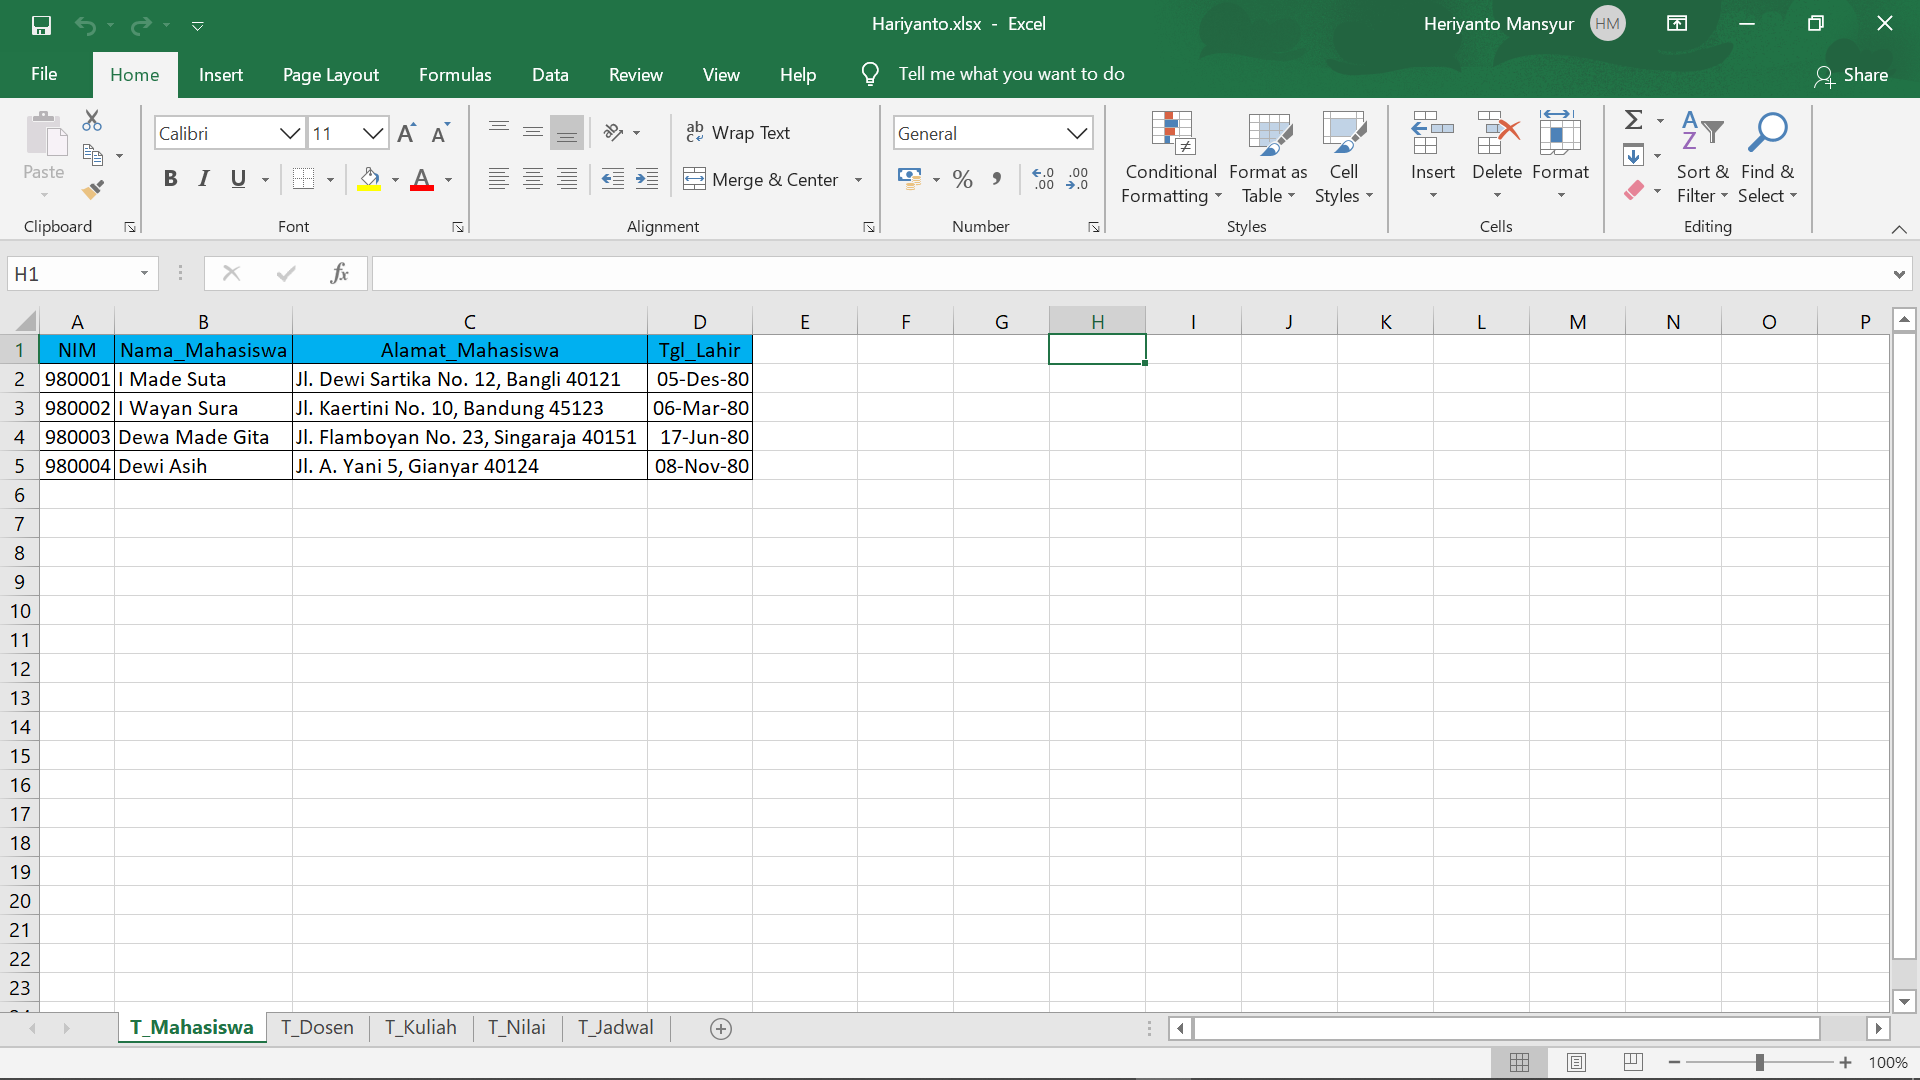
\includegraphics[width=10cm]{figures/Screenshot_27.png}
	\caption{File excel}
\end{figure}
\item Jika sudah ada, silahkan akses ke https://apex.oracle.com/pls/apex/, lalu masukkan workspace, username, dan password sesuai dengan yang anda miliki.
\begin{figure}[htbp]
	\centering
	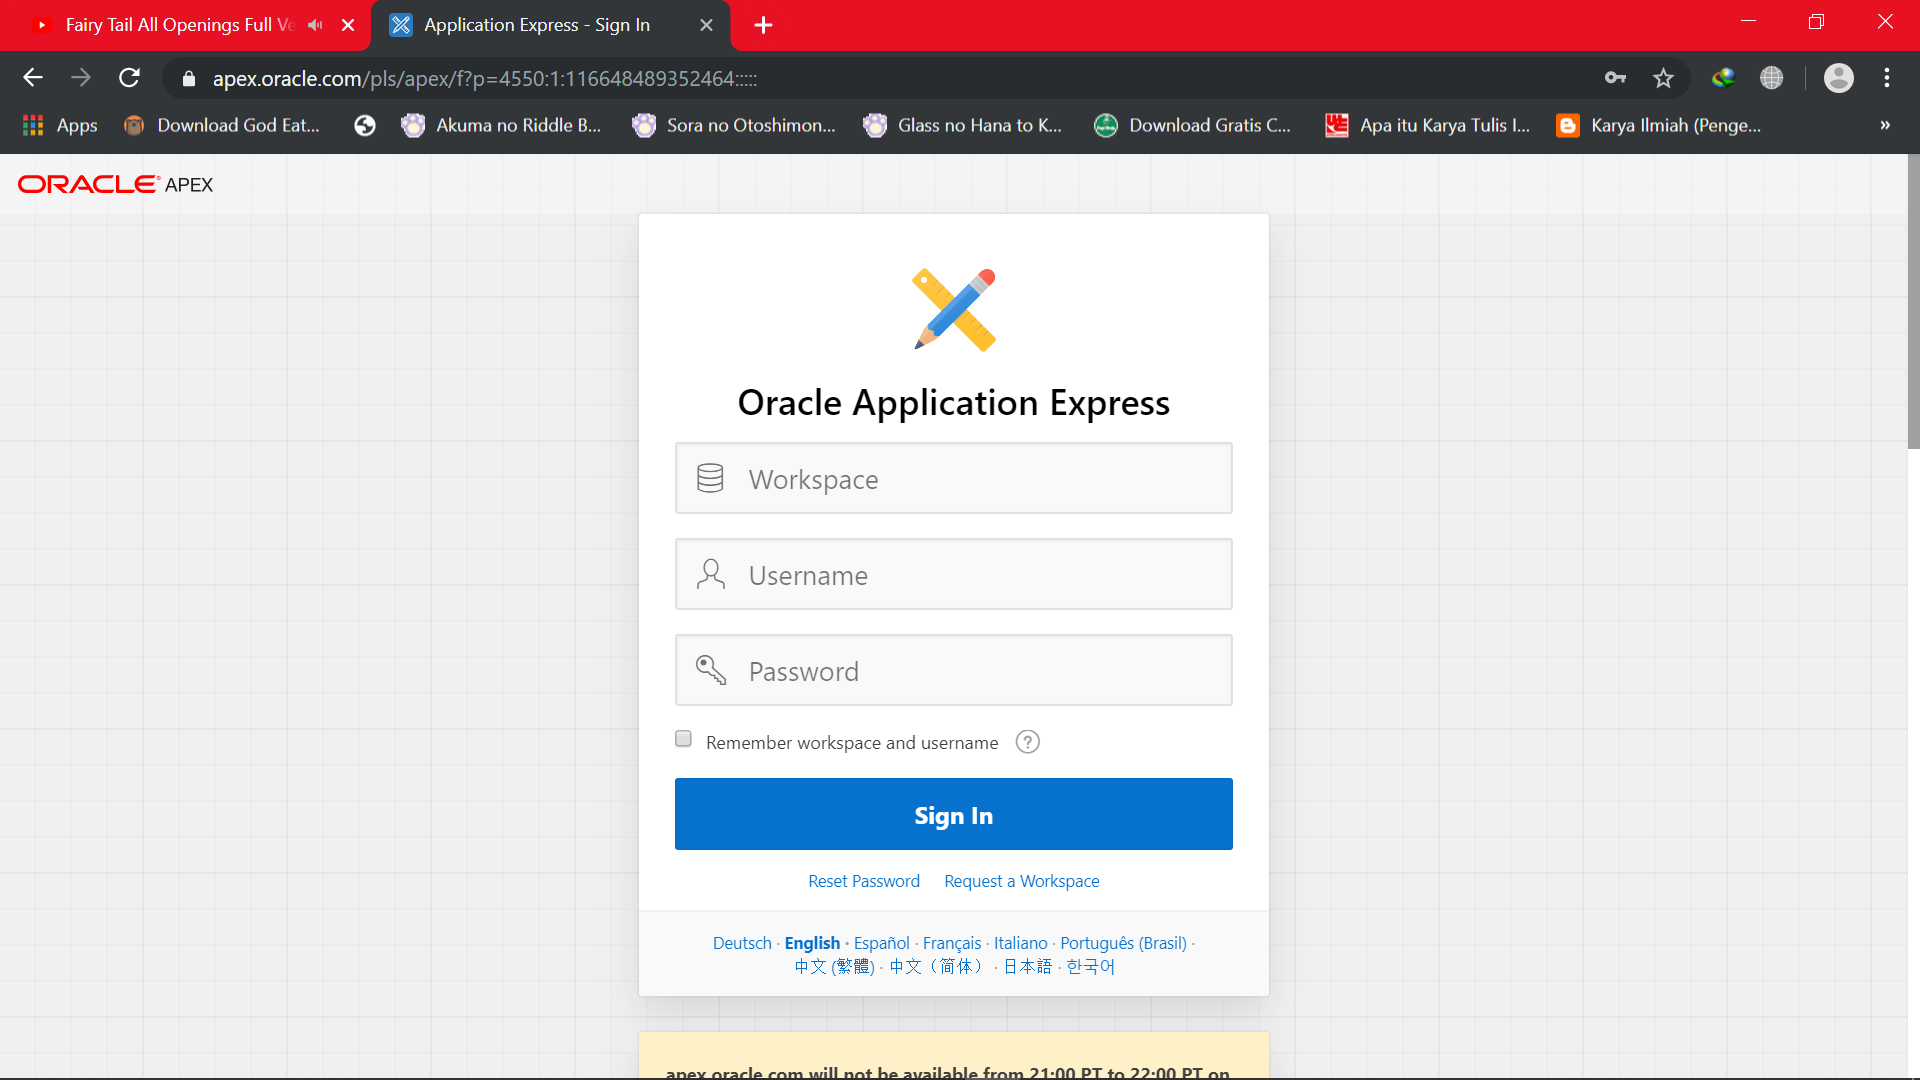
\includegraphics[width=10.5cm]{figures/2.png}
	\caption{Login ke Apex Oracle}
\end{figure}
\item Pada halaman utama apex oracle klik tombol "App Builder" untuk membuat aplikasi.
\begin{figure}[htbp]
	\centering
	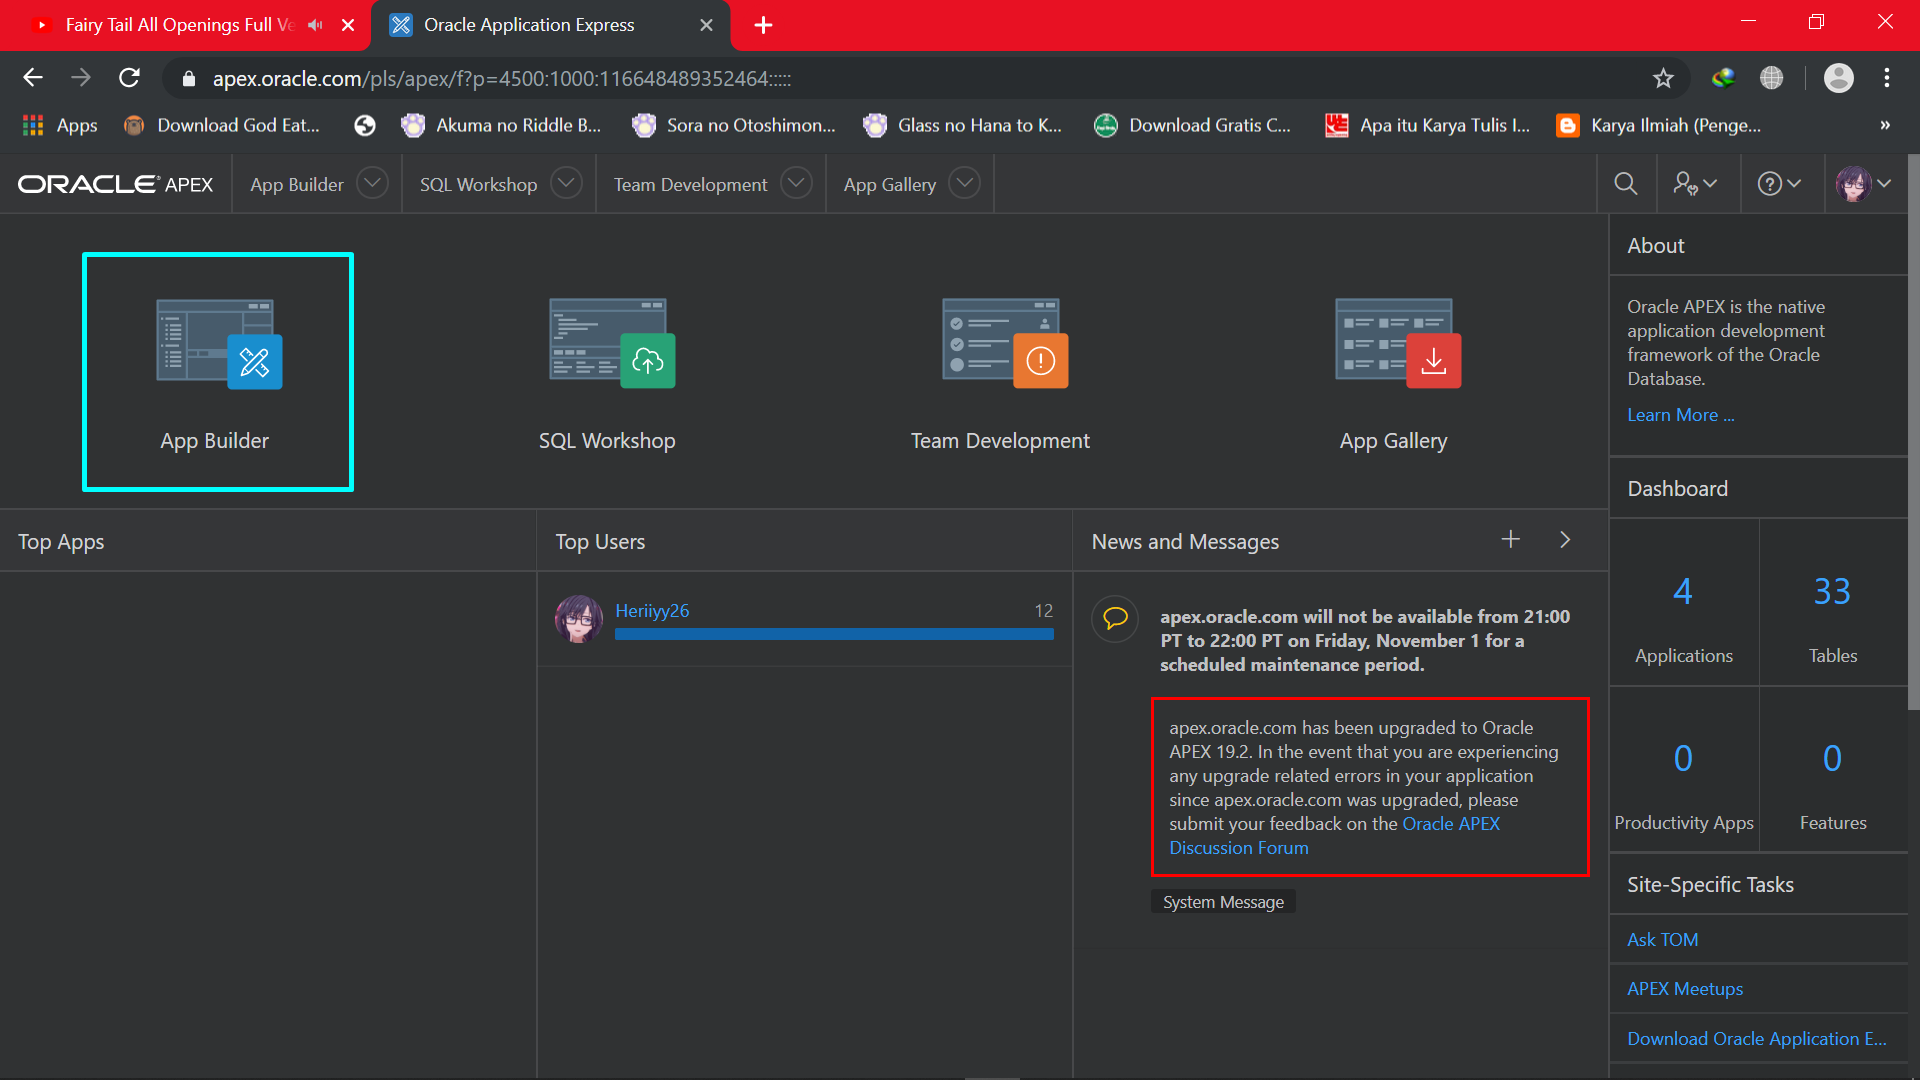
\includegraphics[width=10.5cm]{figures/3.png}
	\caption{Membuka App Builder}
\end{figure}\\
\\
\item Pada halaman App Builder klik tombol "Create" untuk memulai membuat aplikasi.
\begin{figure}[htbp]
	\centering
	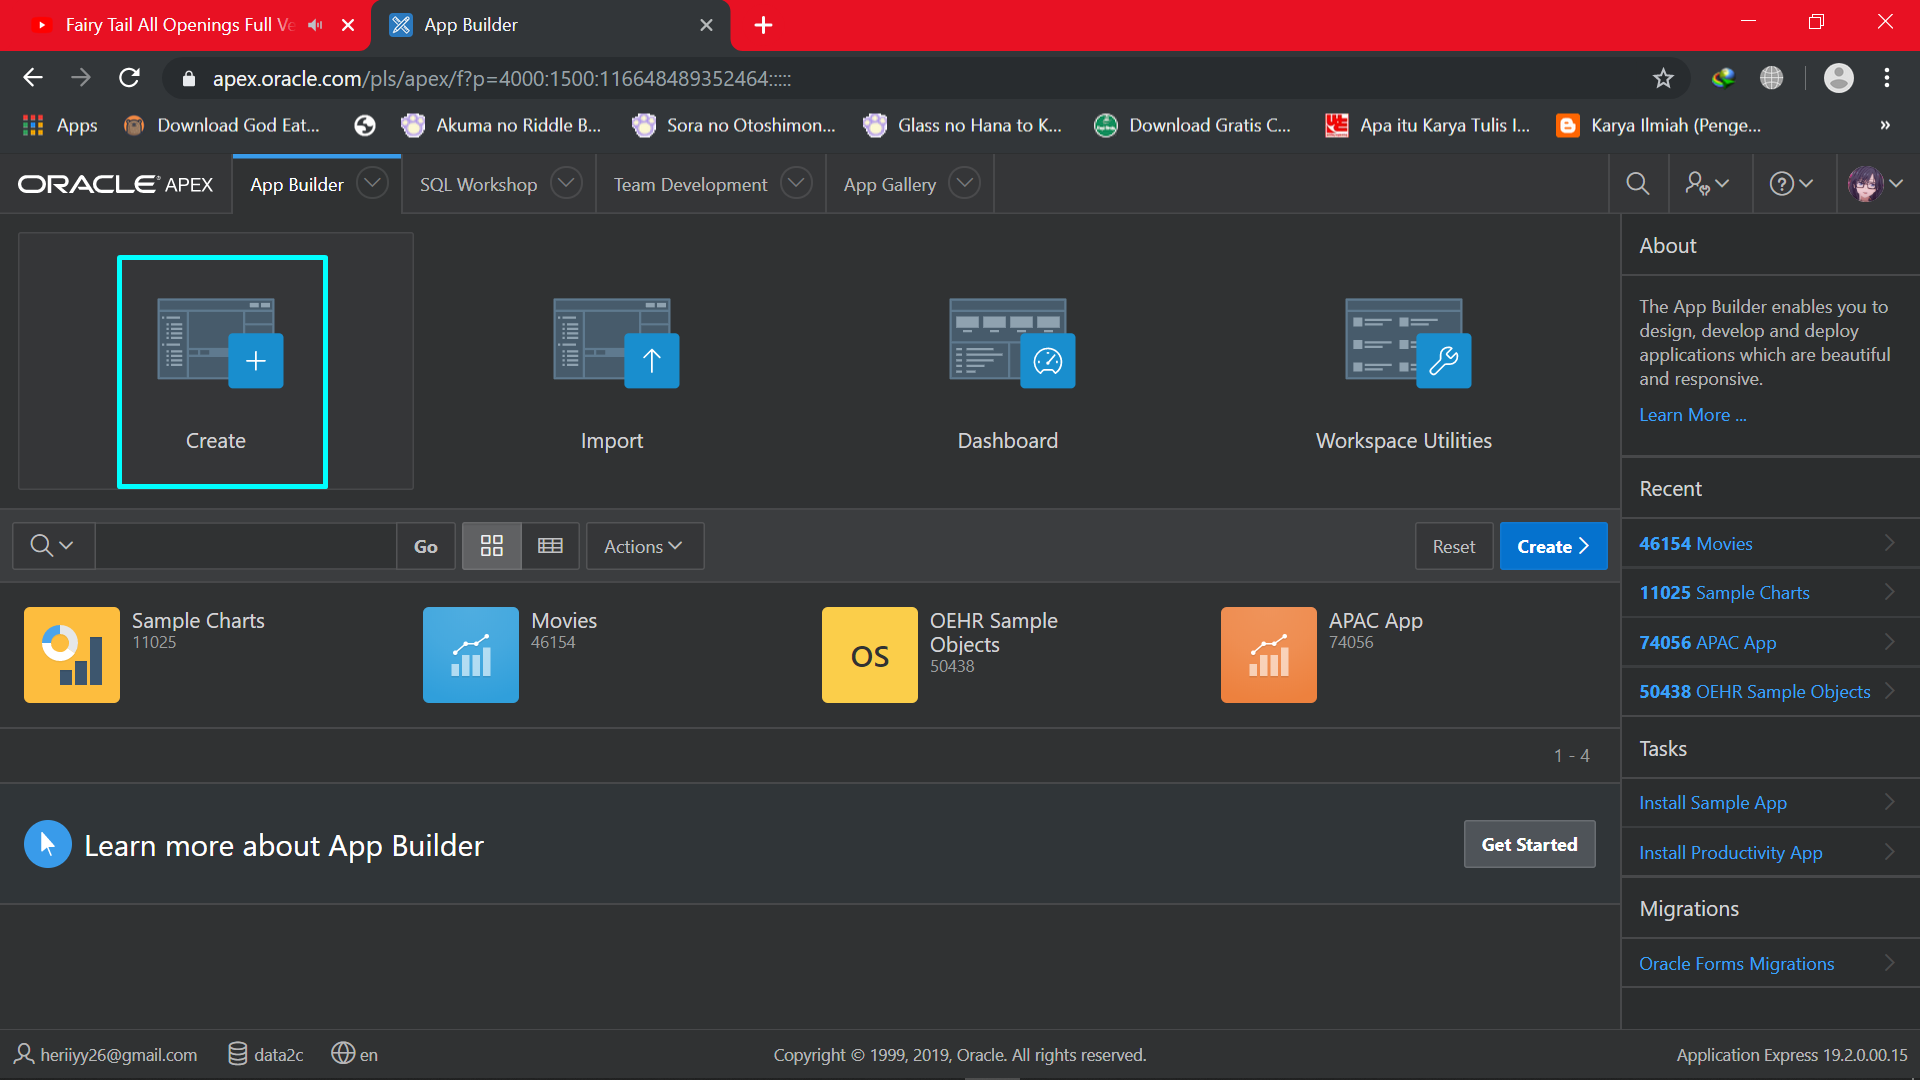
\includegraphics[width=10.5cm]{figures/4.png}
	\caption{Memulai membuat Aplikasi}
\end{figure}
\item Pada halaman Create Application ada tiga fitur dalam membuat aplikasi, disini kita akan memakai fitur "From a File" dari file excel kita tadi, jadi silahkan klik.
\begin{figure}[htbp]
	\centering
	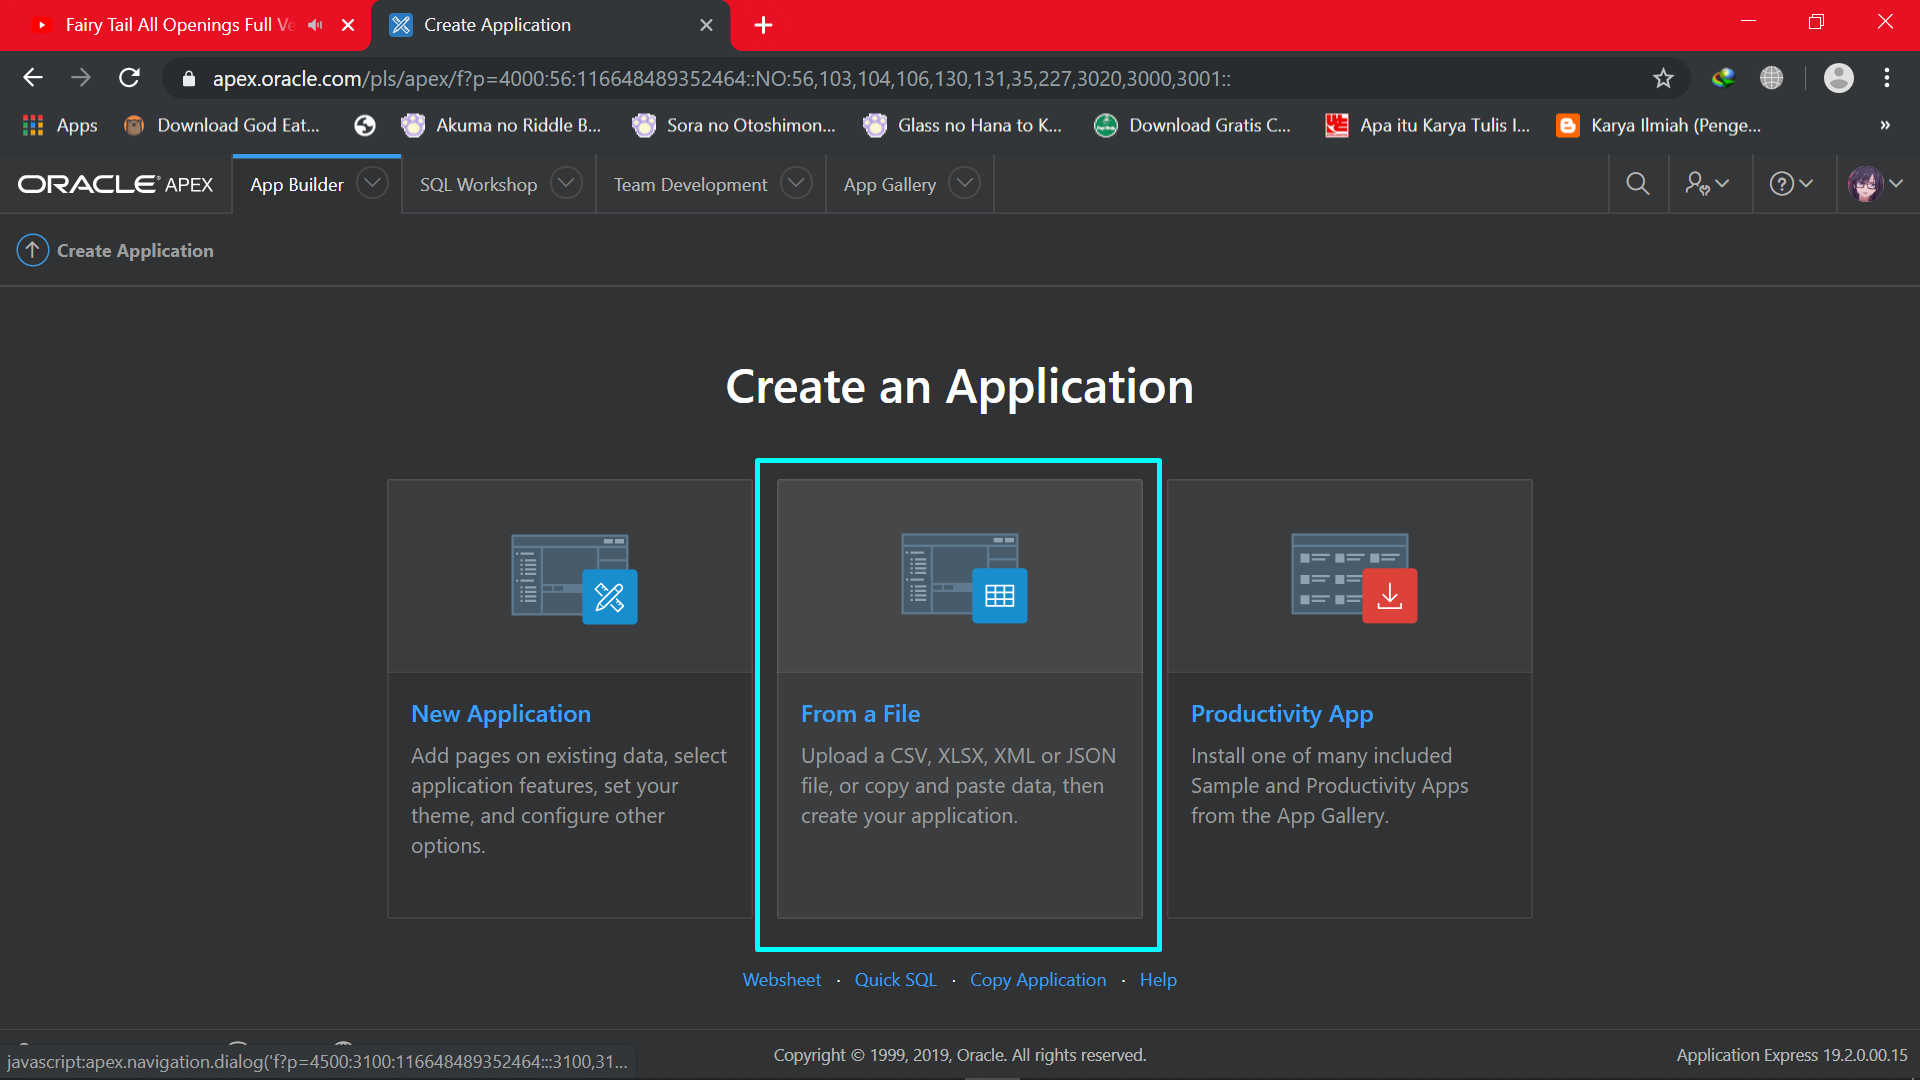
\includegraphics[width=10.5cm]{figures/5.png}
	\caption{Membuat aplikasi dari file}
\end{figure}\\
\\
\item Setelah di-klik akan muncul dialog load data, di dialog tersebut pilih tab "Upload a File" lalu klik tombol "Choose File".
\begin{figure}[htbp]
	\centering
	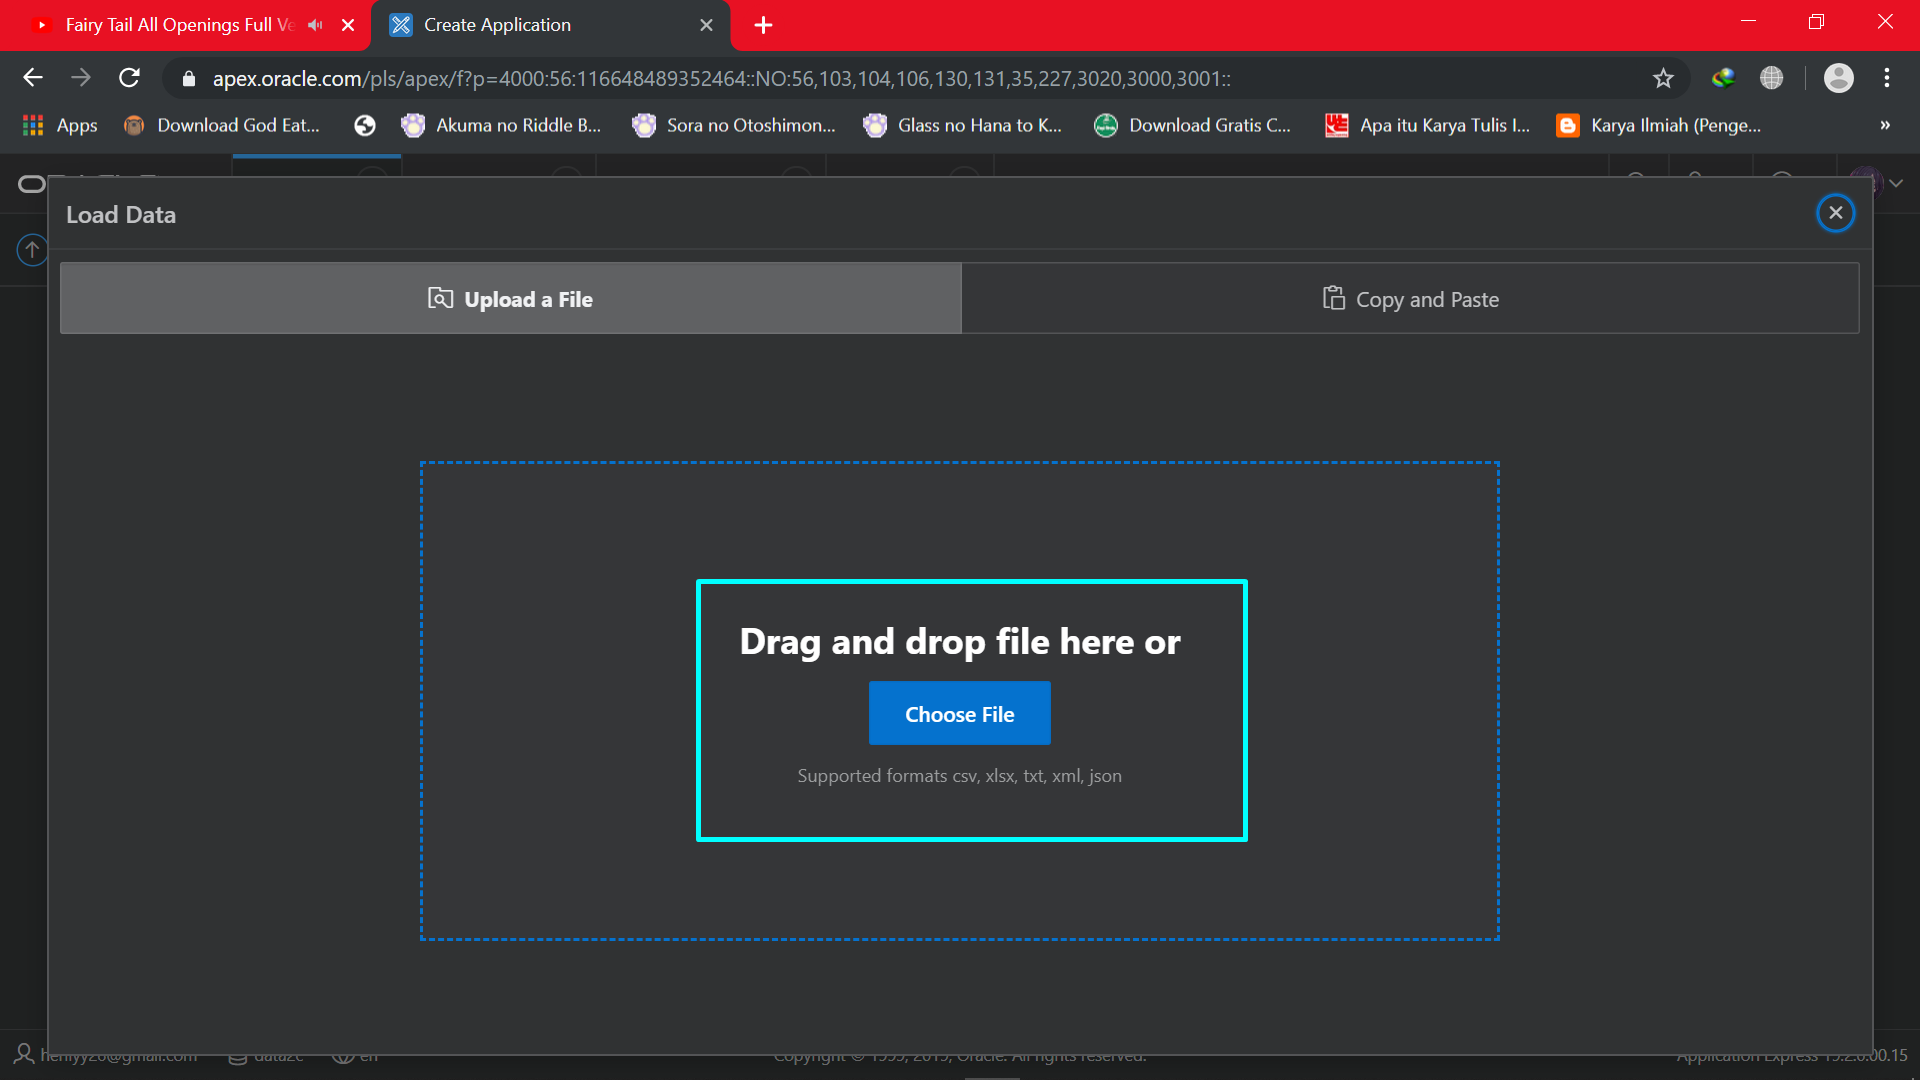
\includegraphics[width=10.5cm]{figures/6.png}
	\caption{Meng-upload file}
\end{figure}
\item Buka tempat dimana file excel anda tersimpan, disini file saya adalah Hariyanto.xlsx.
\begin{figure}[htbp]
	\centering
	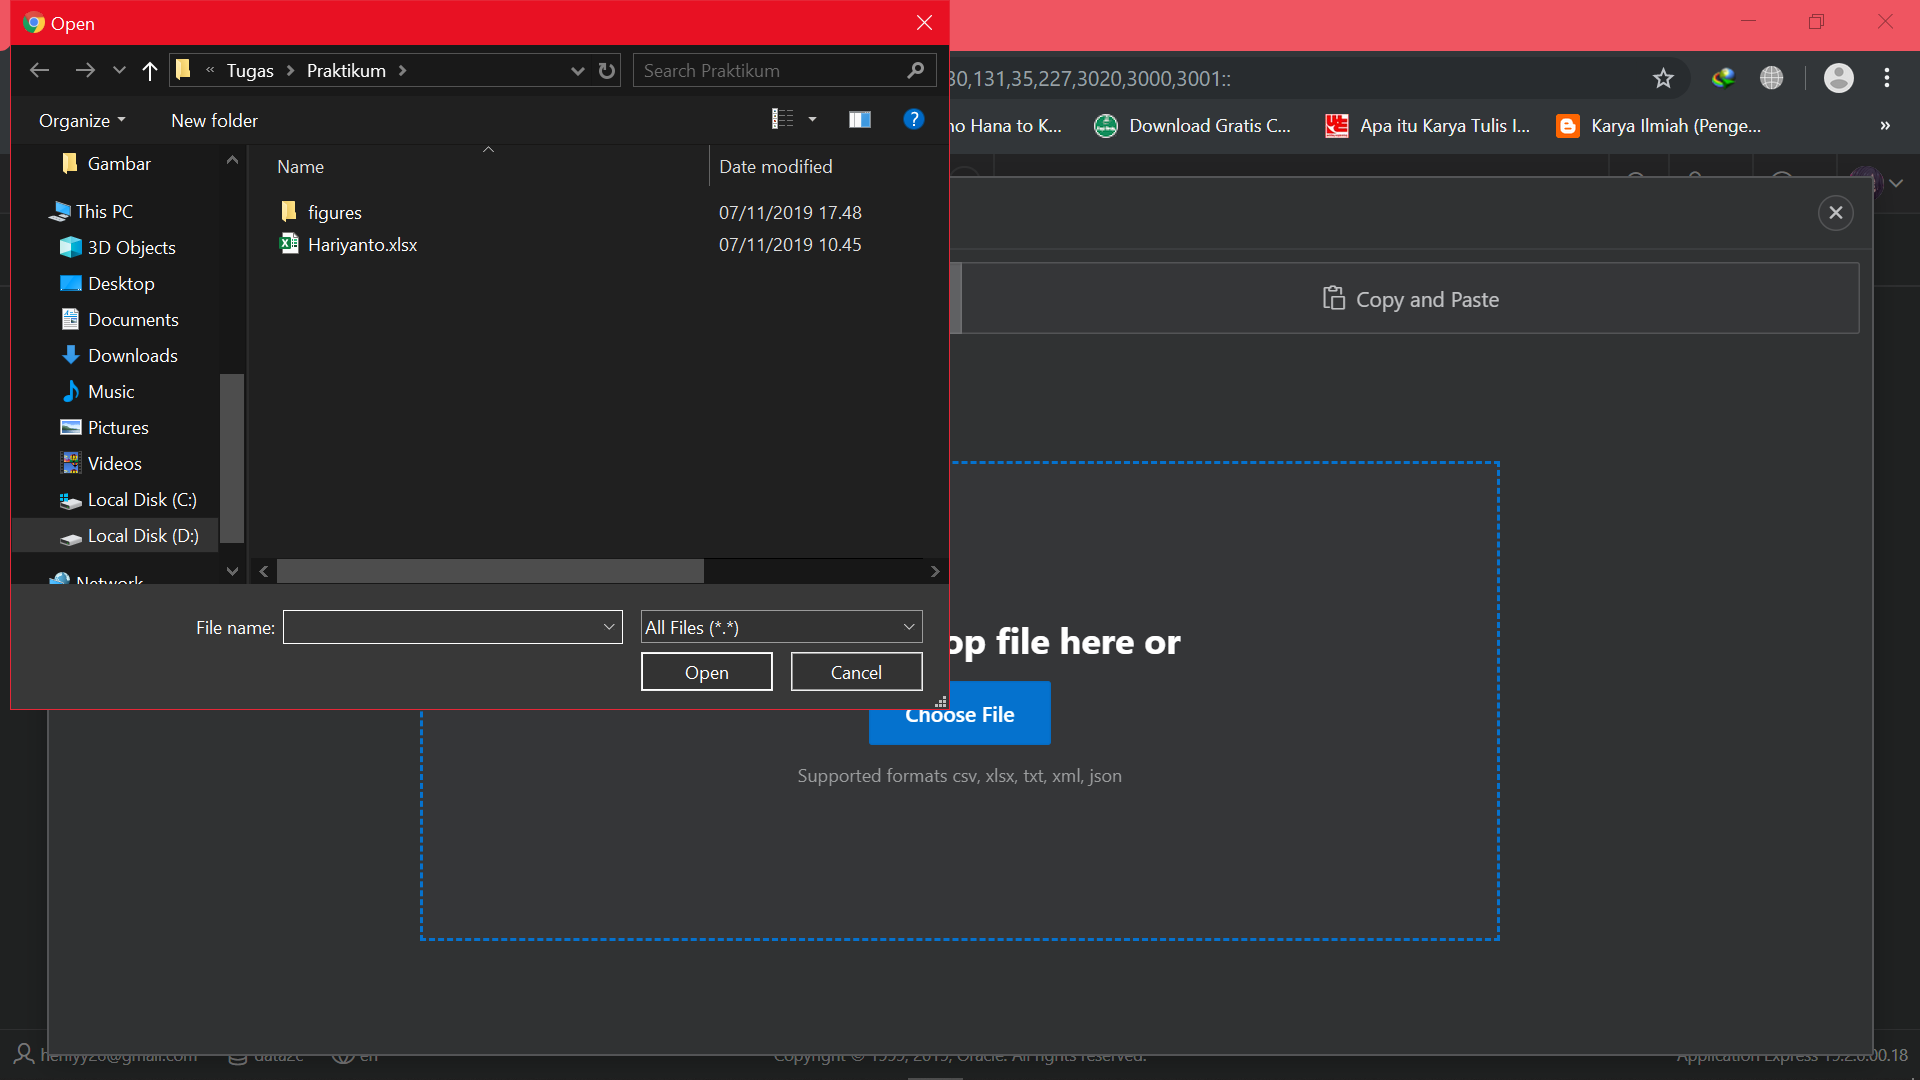
\includegraphics[width=10.5cm]{figures/Screenshot_5.png}
	\caption{Membuka tempat file disimpan}
\end{figure}\\
\\
\\
\item JIka sudah silahkan isi nama tabel dengan nama "TMahasiswa". 
\begin{figure}[htbp]
	\centering
	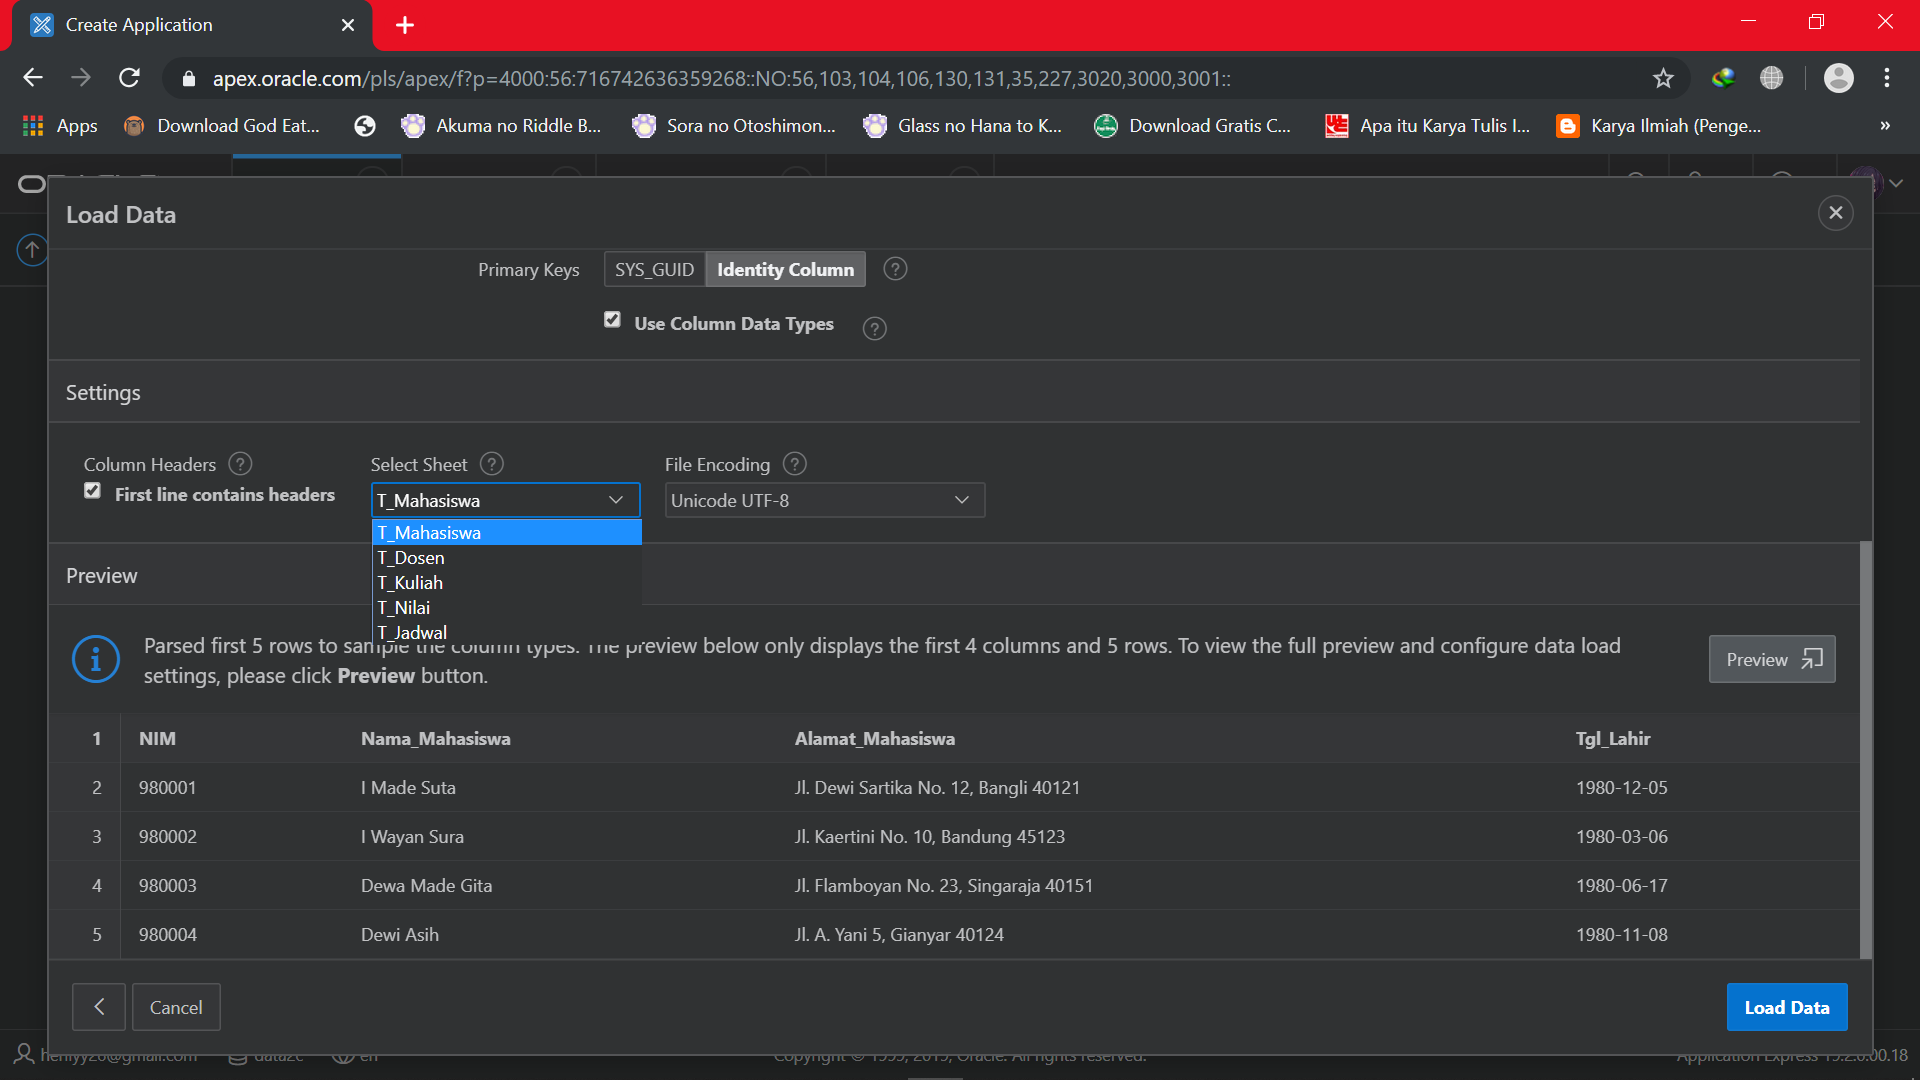
\includegraphics[width=10.5cm]{figures/Screenshot_6.png}
	\caption{Memberi nama tabel}
\end{figure}
\item Scroll ke bawah dan pilih sheets "TMAHASISWA". Lalu load data dan ulang untuk sheets lainnya.
\begin{figure}[htbp]
	\centering
	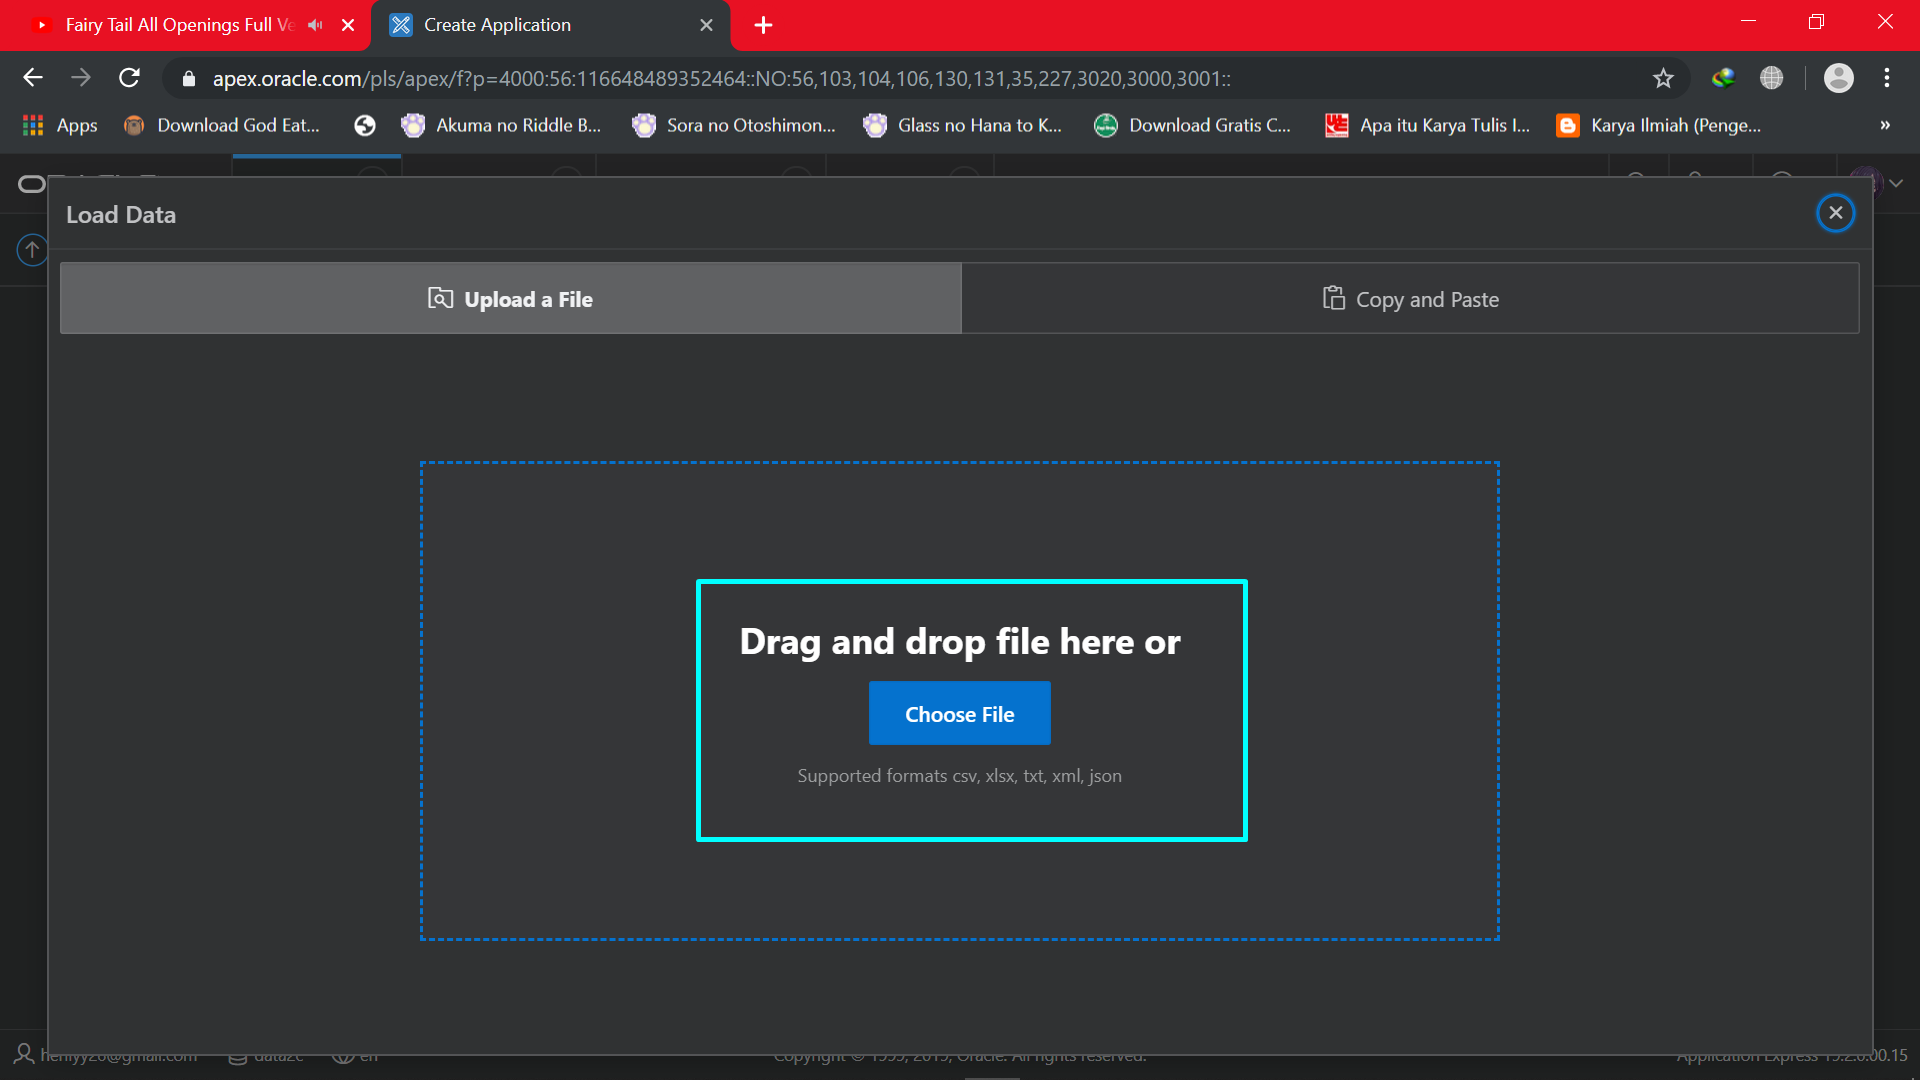
\includegraphics[width=10.5cm]{figures/6.png}
	\caption{Load Data}
\end{figure}\\
\\
\item Jika sudah kita akan normalisasi tabel tersebut. Yang pertama adalah primary key untuk tabel mahasiswa. Lakukan cara yang sama untuk tabel dosen dan tabel kuliah saja.
\begin{figure}[htbp]
	\centering
	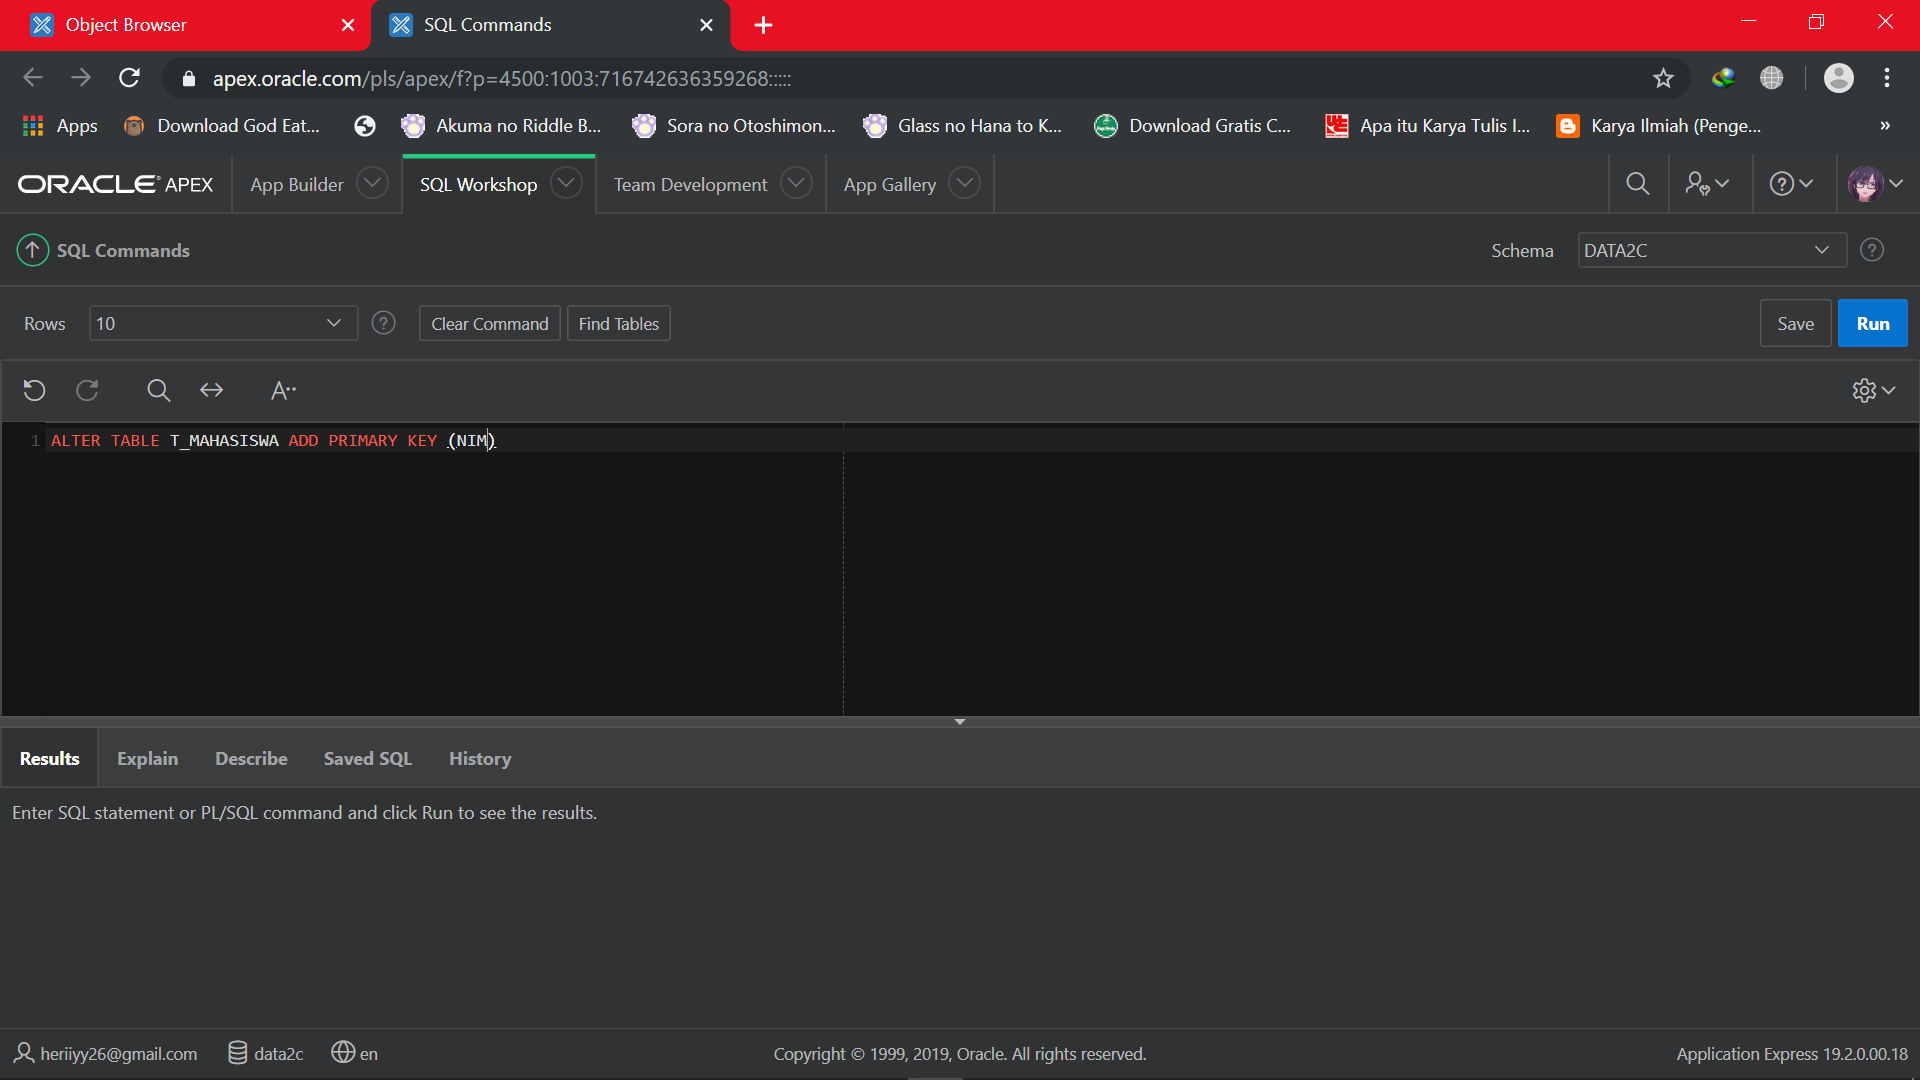
\includegraphics[width=10.5cm]{figures/Screenshot_7.png}
	\caption{Primary Key}
\end{figure}
\item Kedua adalah memberi foreign key kode tabel kuliah ke tabel nilai.
\begin{figure}[htbp]
	\centering
	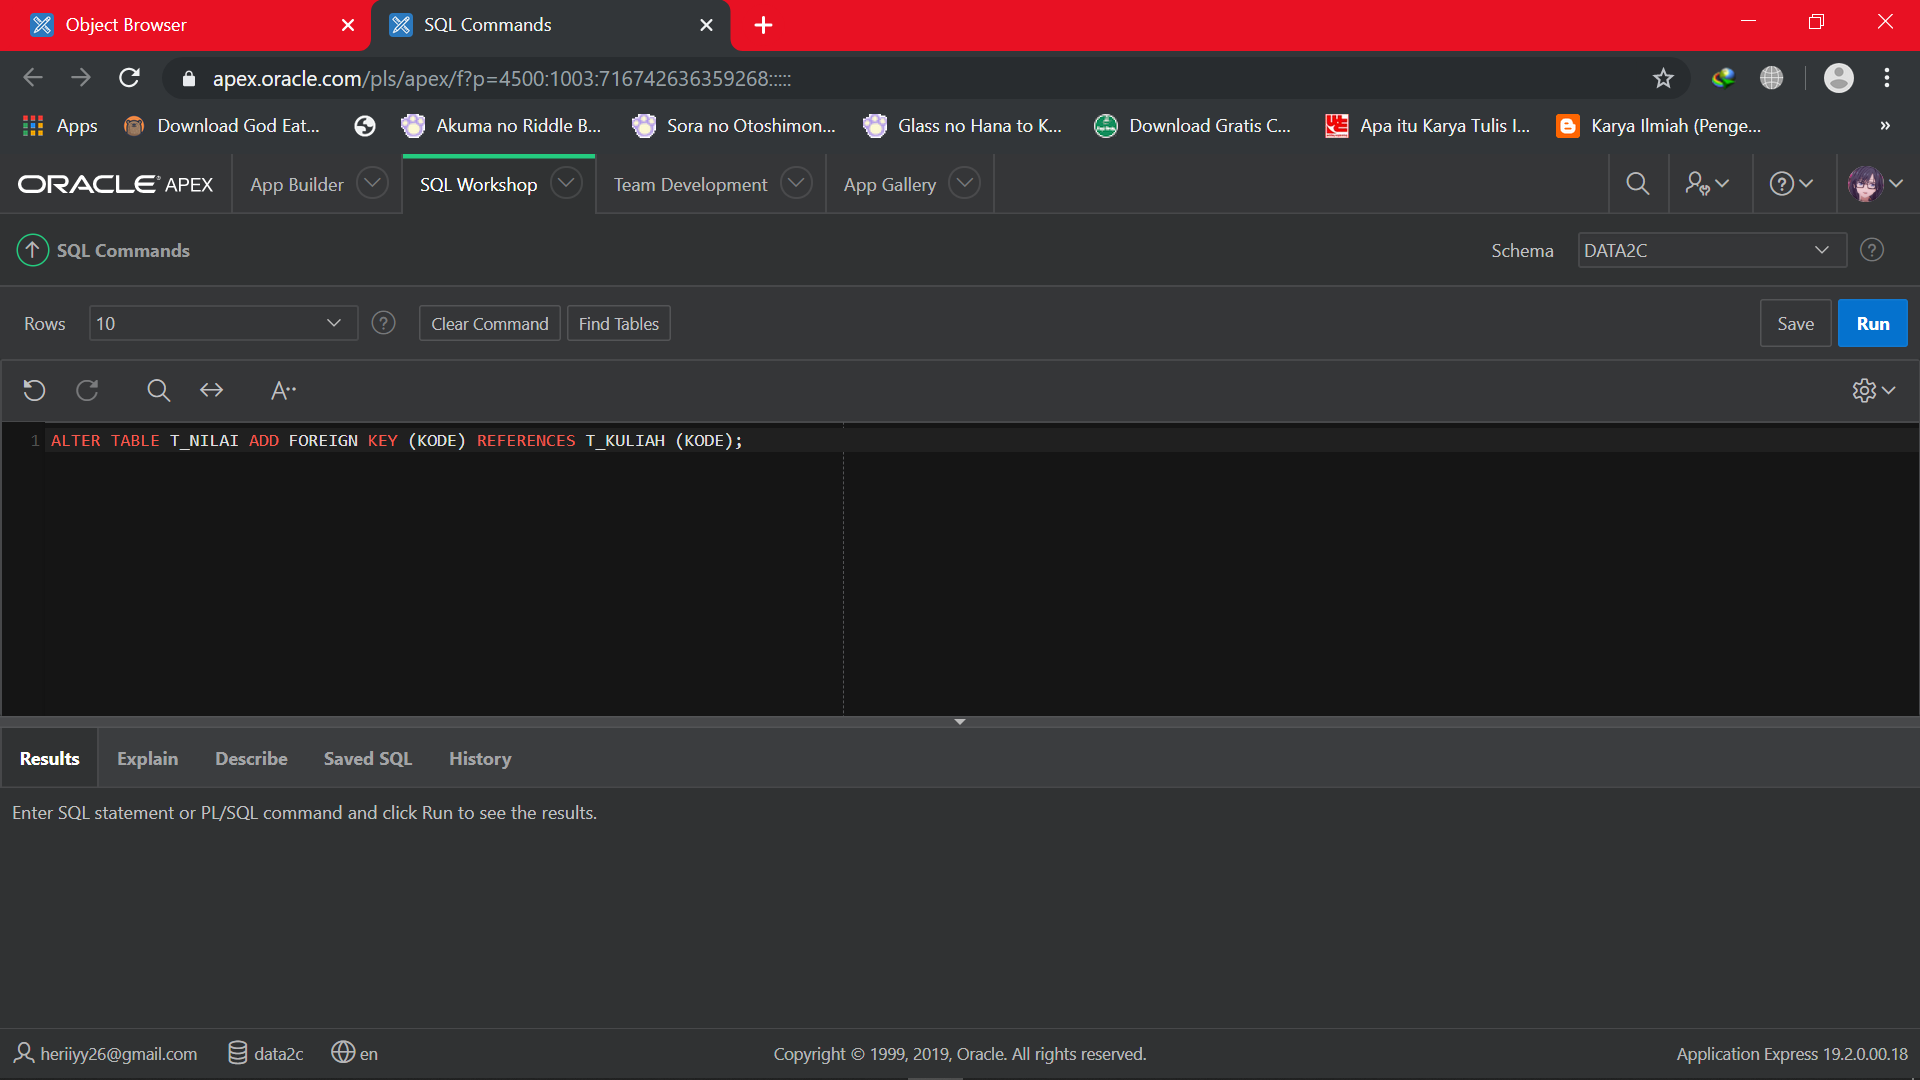
\includegraphics[width=10.5cm]{figures/Screenshot_8.png}
	\caption{Foreign Key}
\end{figure}\\
\\
\item Ketiga adalah memberi foreign key nim tabel mahasiswa ke tabel nilai.
\begin{figure}[htbp]
	\centering
	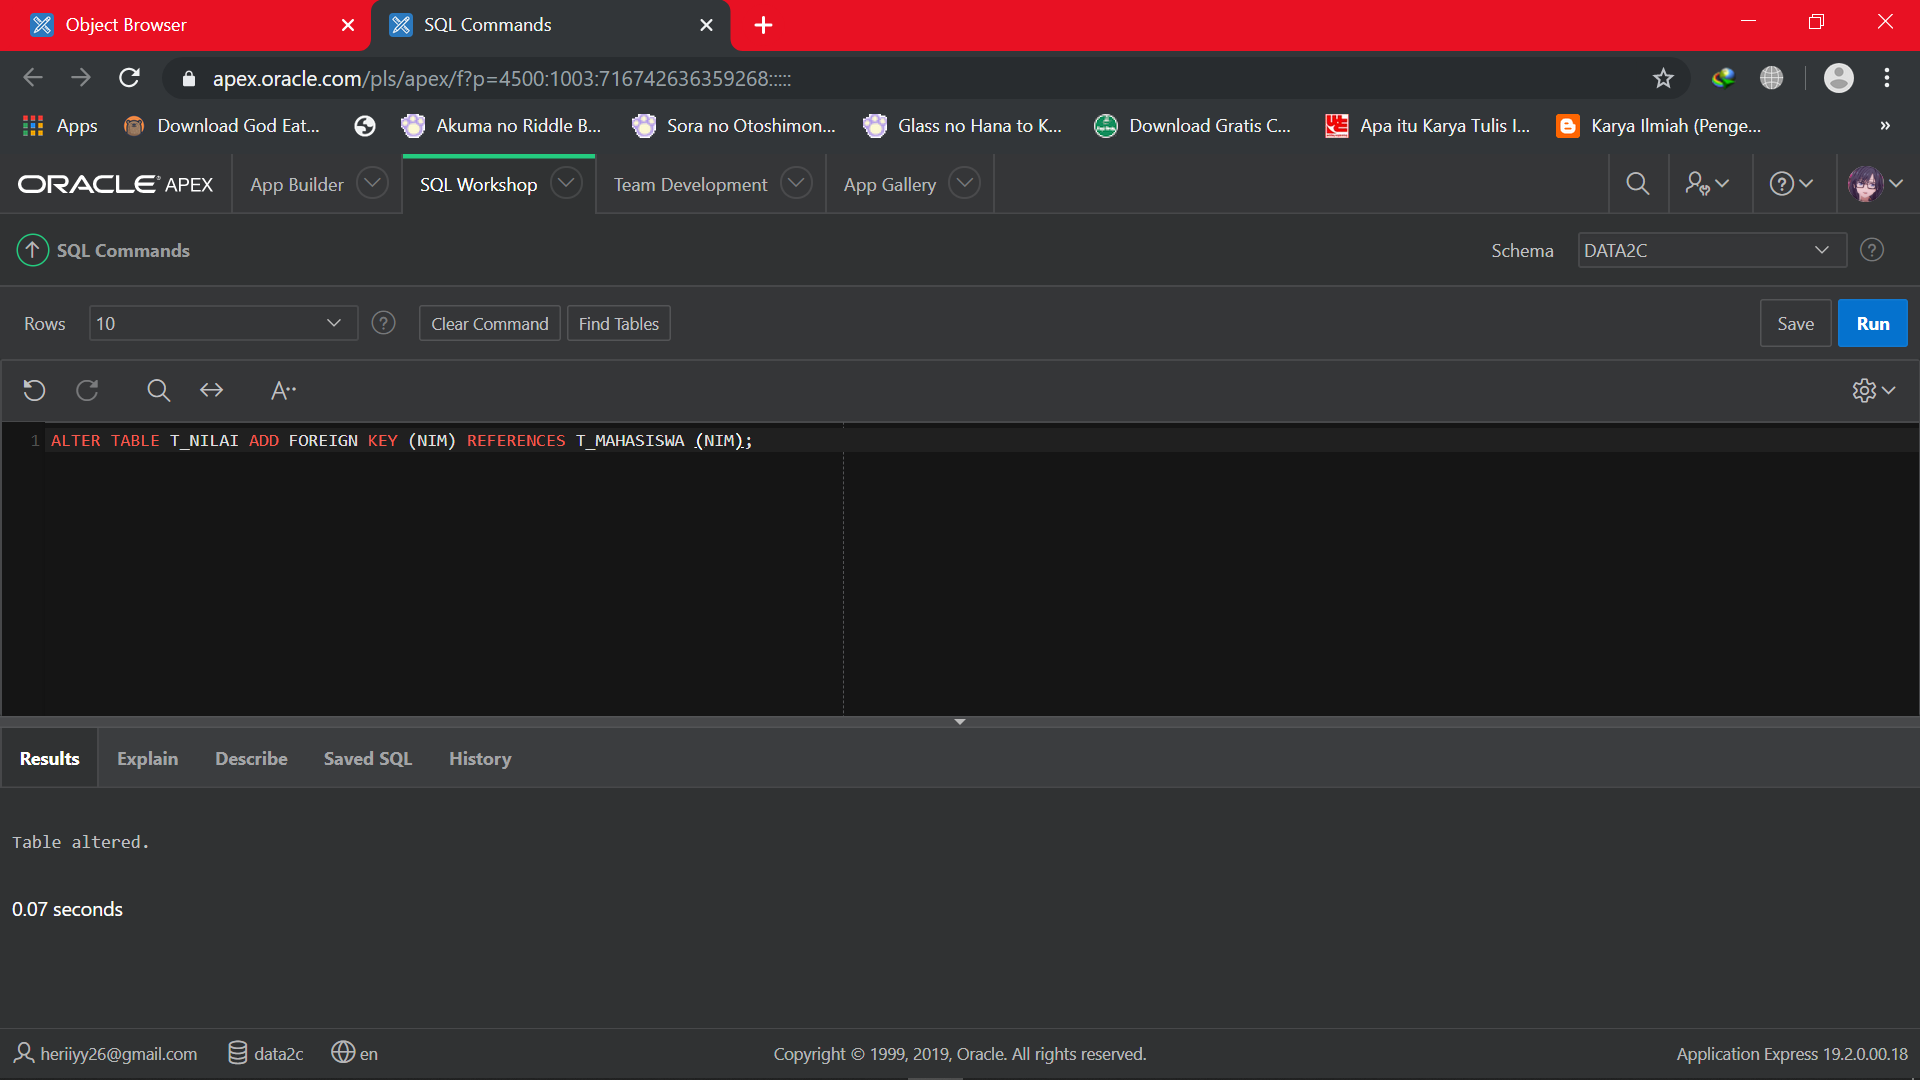
\includegraphics[width=10.5cm]{figures/Screenshot_9.png}
	\caption{Foreign Key}
\end{figure}
\item Keempat adalah memberi foreign key nik dari tabel dosen ke tabel jadwal.
\begin{figure}[htbp]
	\centering
	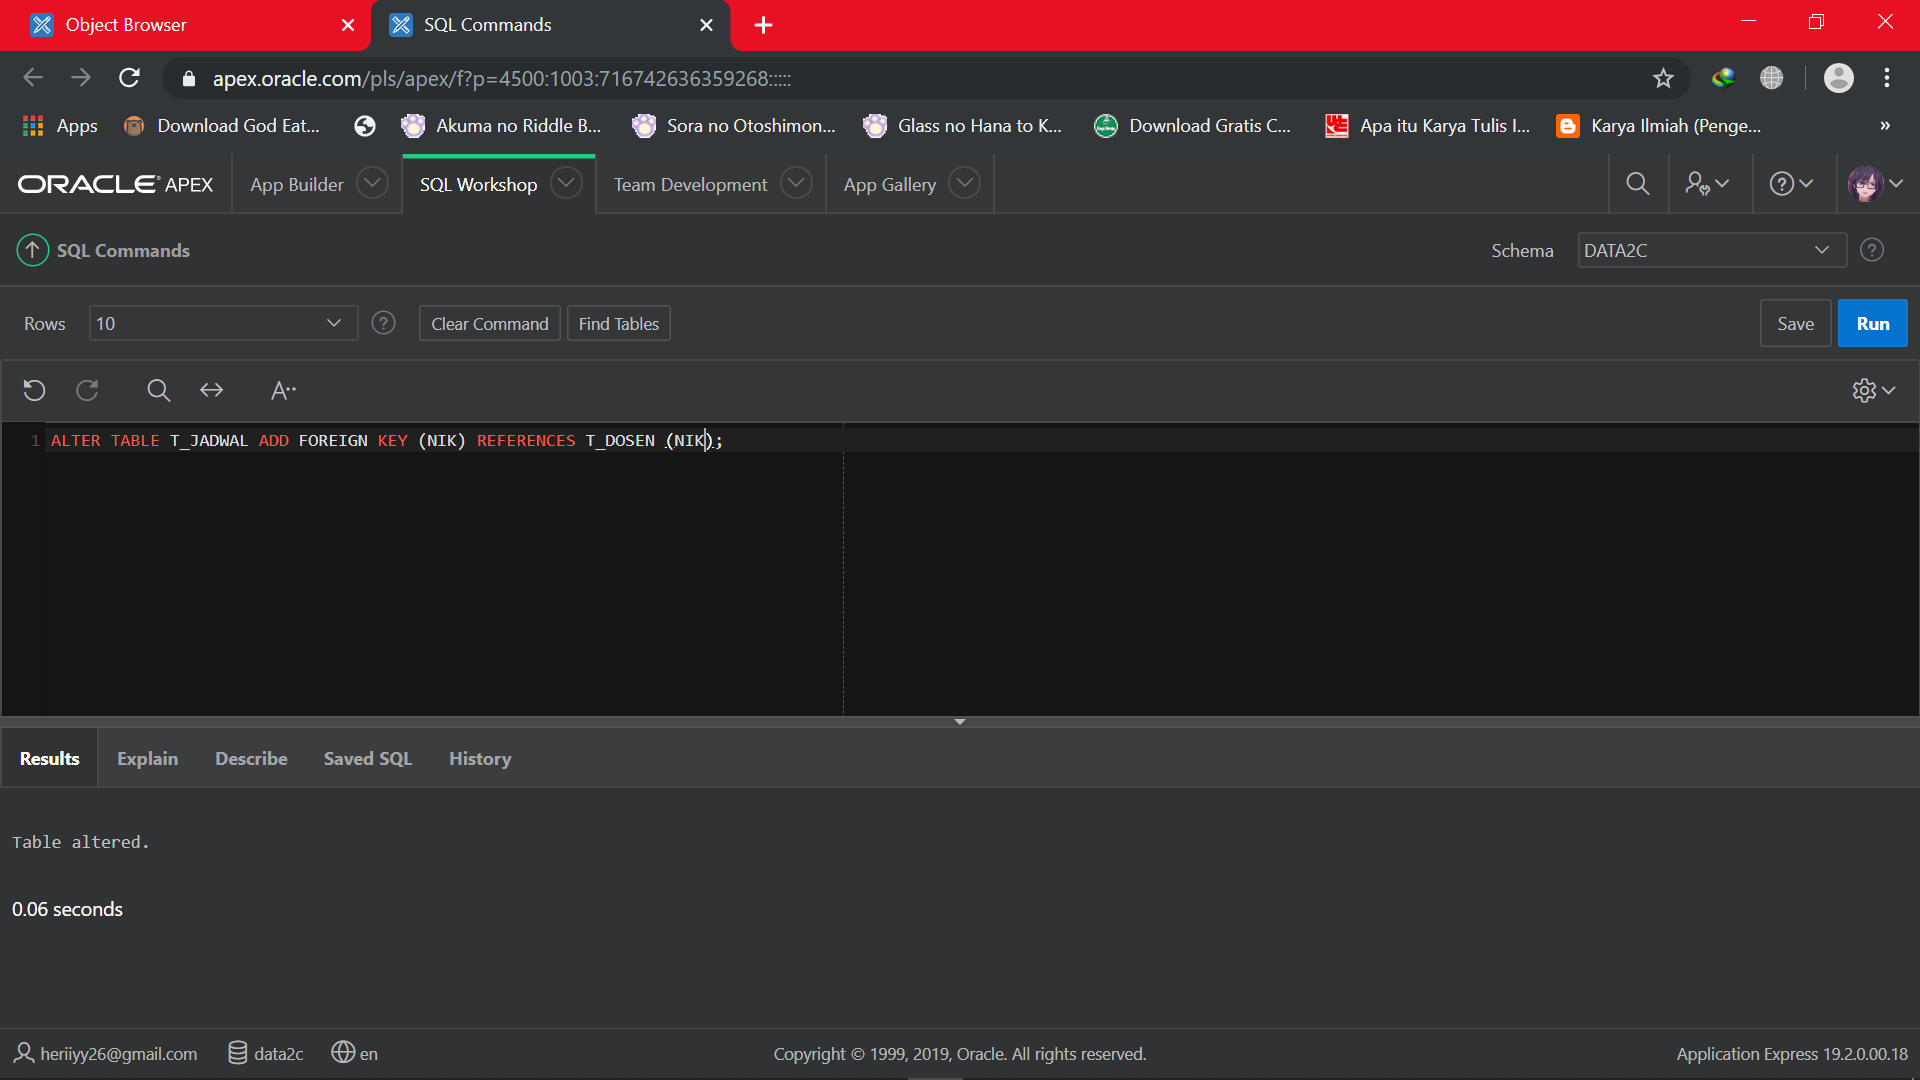
\includegraphics[width=10.5cm]{figures/Screenshot_10.png}
	\caption{Foreign Key}
\end{figure}\\
\\
\item Terakhir adalah memberi foreign key dari kode tabel kuliah ke tabel jadwal.
\begin{figure}[htbp]
	\centering
	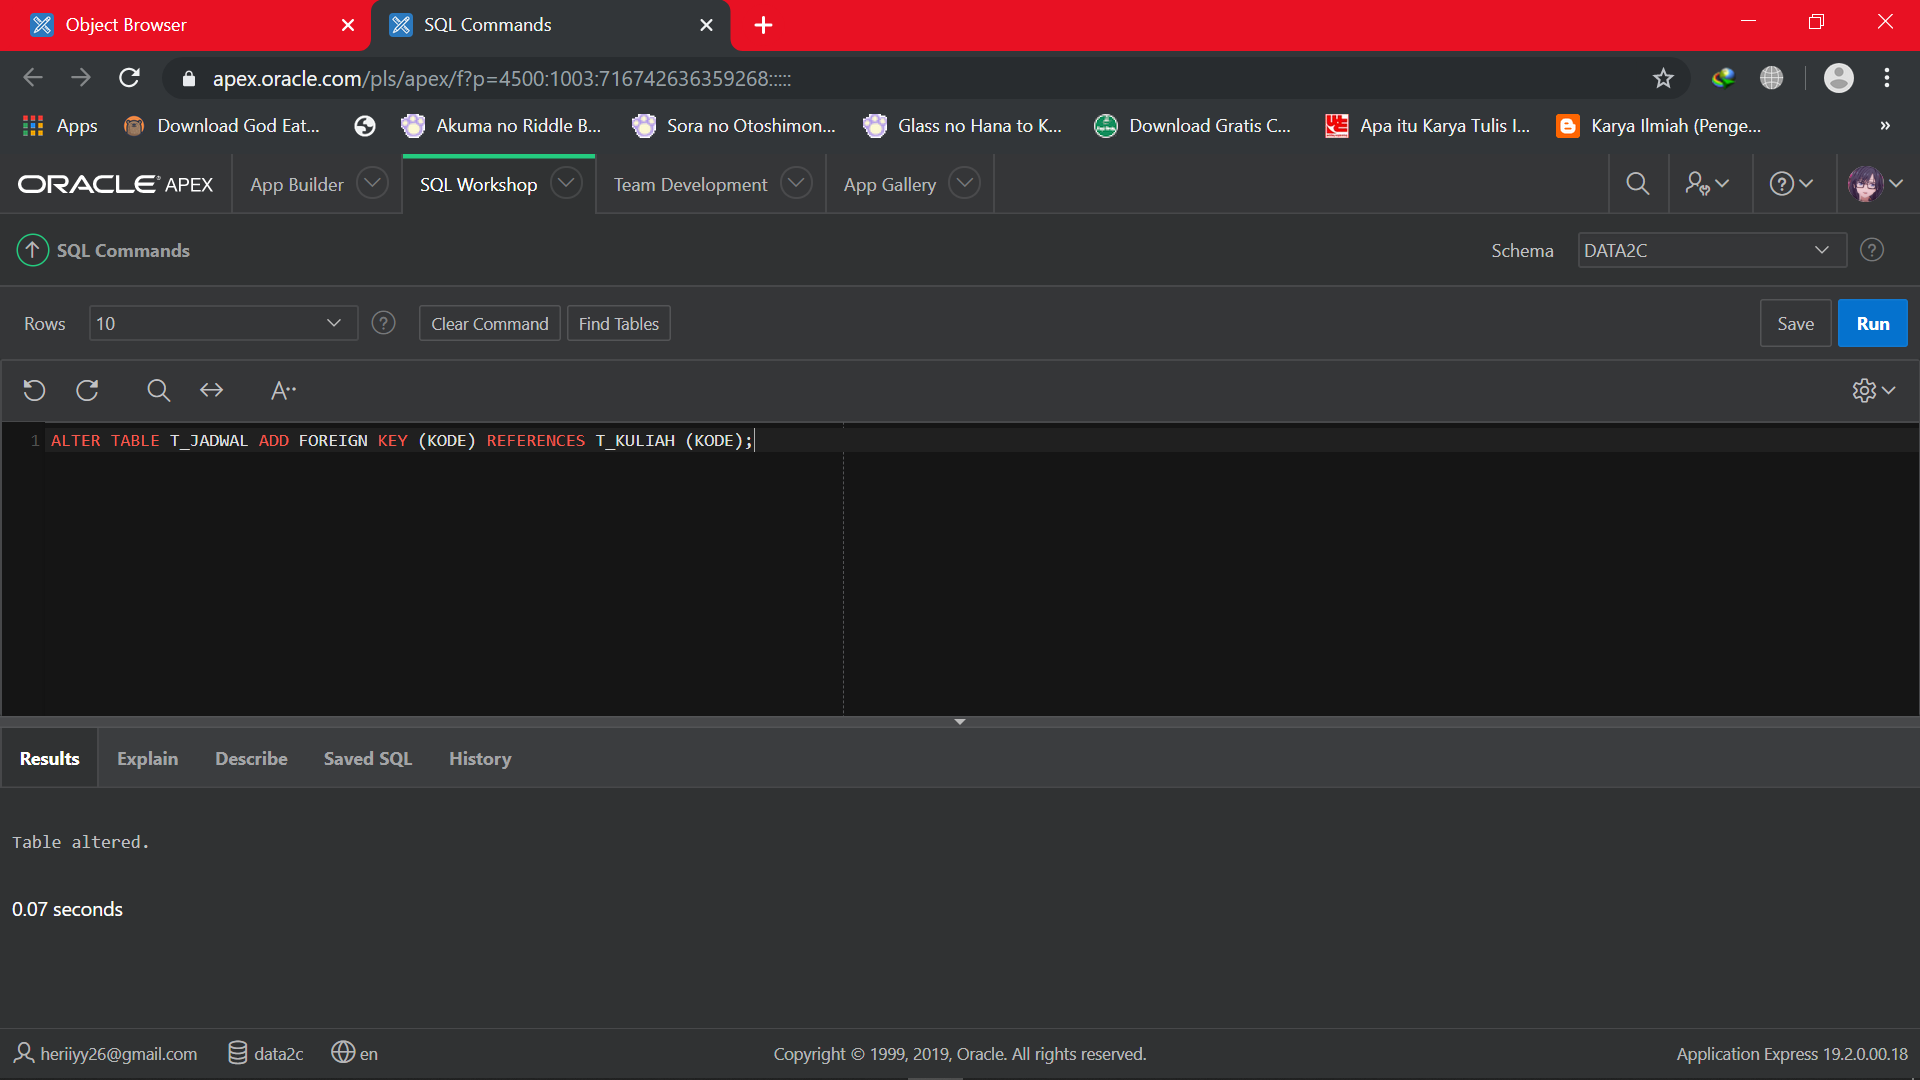
\includegraphics[width=10.5cm]{figures/Screenshot_11.png}
	\caption{Foreign Key}
\end{figure}
\item Sekarang kita akan membuat aplikasinya, caranya adalah klik app builder lalu klik "Create".
\begin{figure}[htbp]
	\centering
	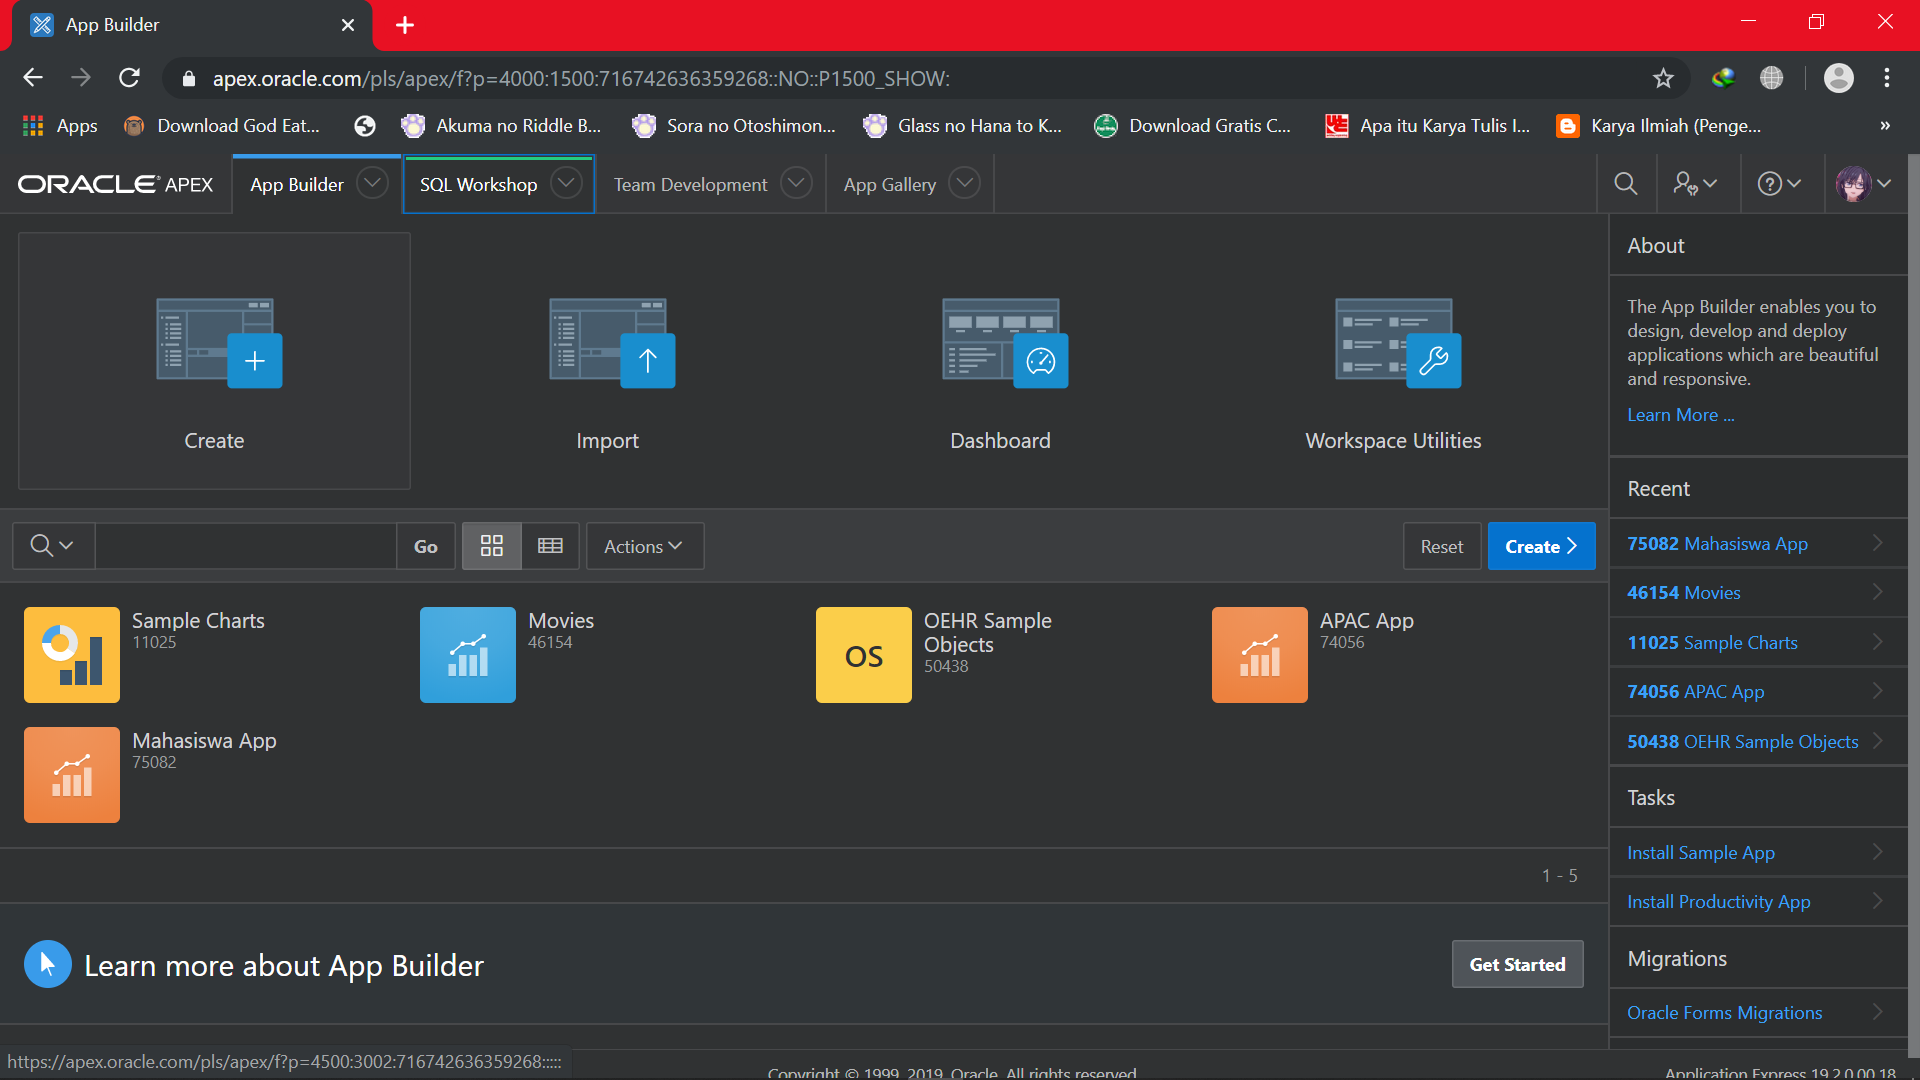
\includegraphics[width=10.5cm]{figures/Screenshot_12.png}
	\caption{Membuat Aplikasi}
\end{figure}\\
\\
\item Selanjutnya akan dialihkan pada halaman Create Application, klik "New Application".
\begin{figure}[htbp]
	\centering
	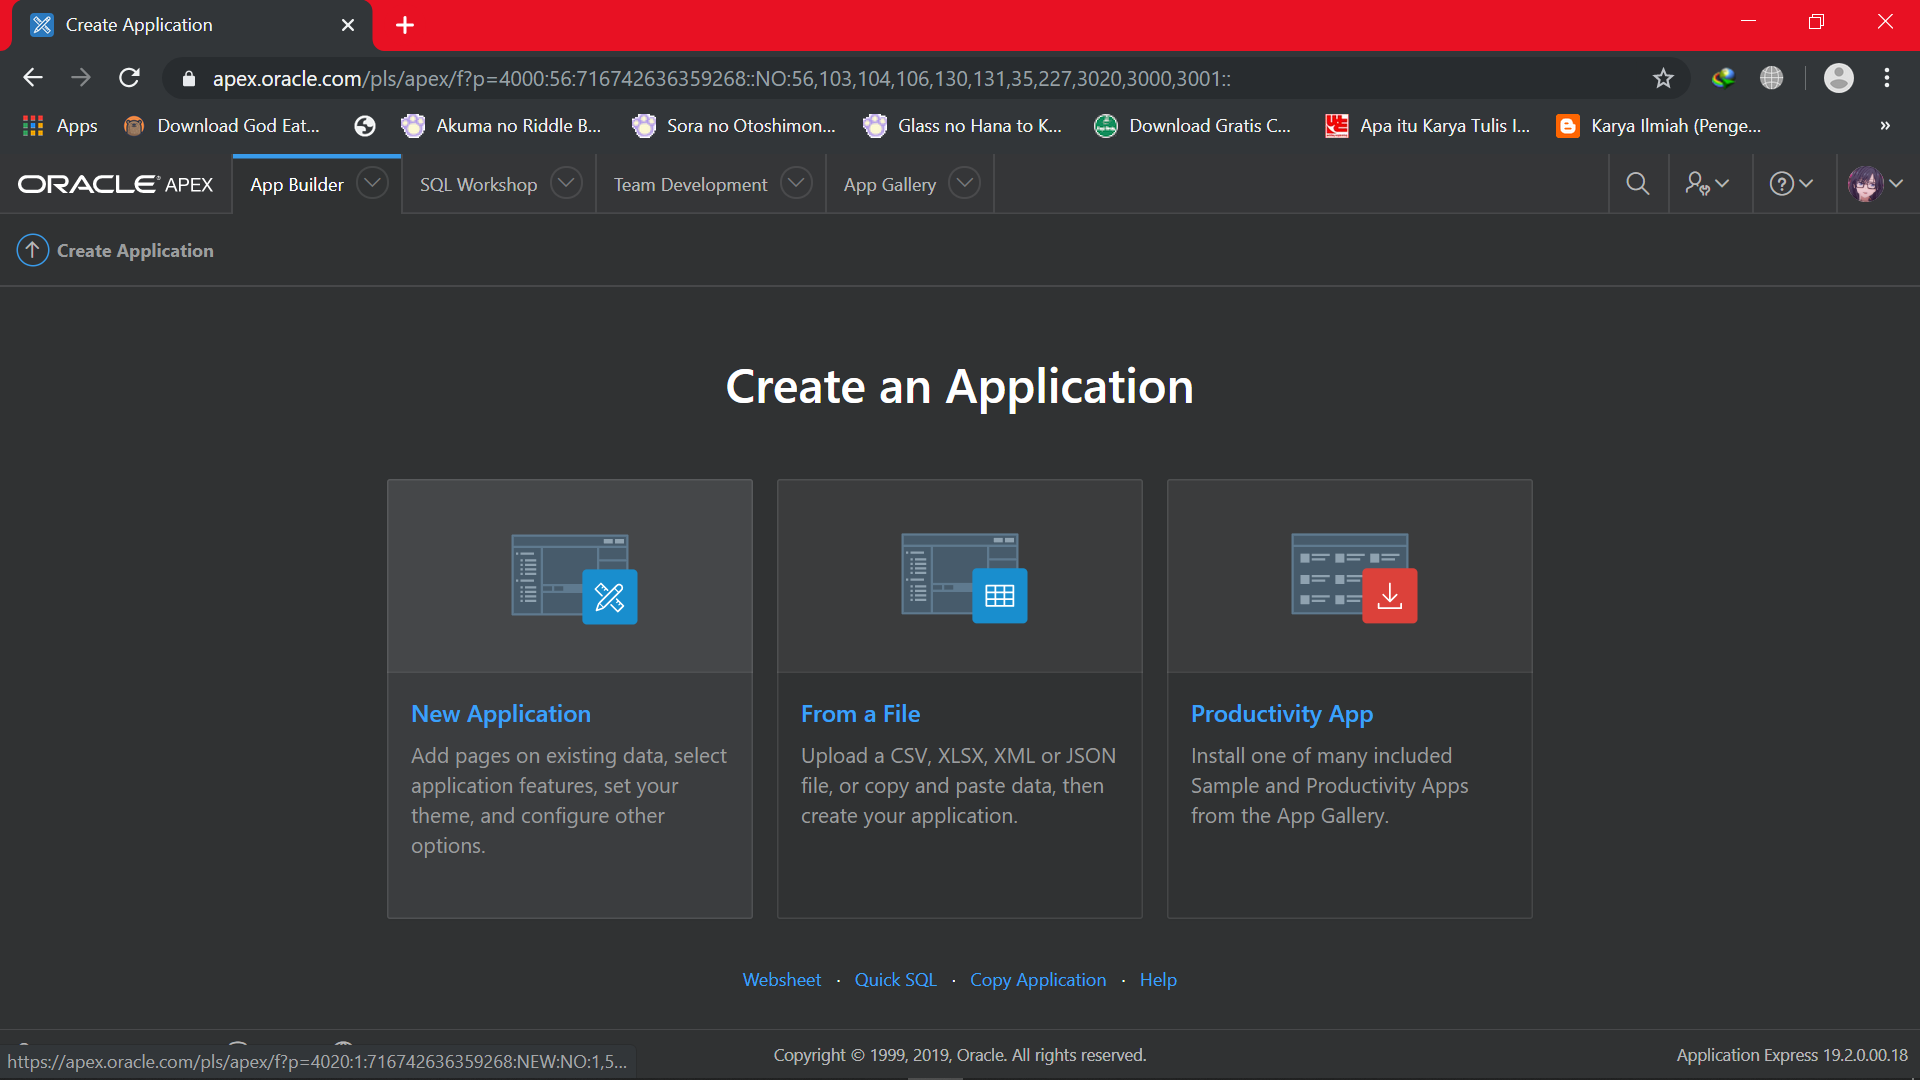
\includegraphics[width=10.5cm]{figures/Screenshot_13.png}
	\caption{Membuat Aplikasi}
\end{figure}
\item Selanjutnya akan dialihkan pada halaman Create an Application, isinya nama aplikasi dengan nama "Perkuliahan App" pada kotak "Name".
\begin{figure}[htbp]
	\centering
	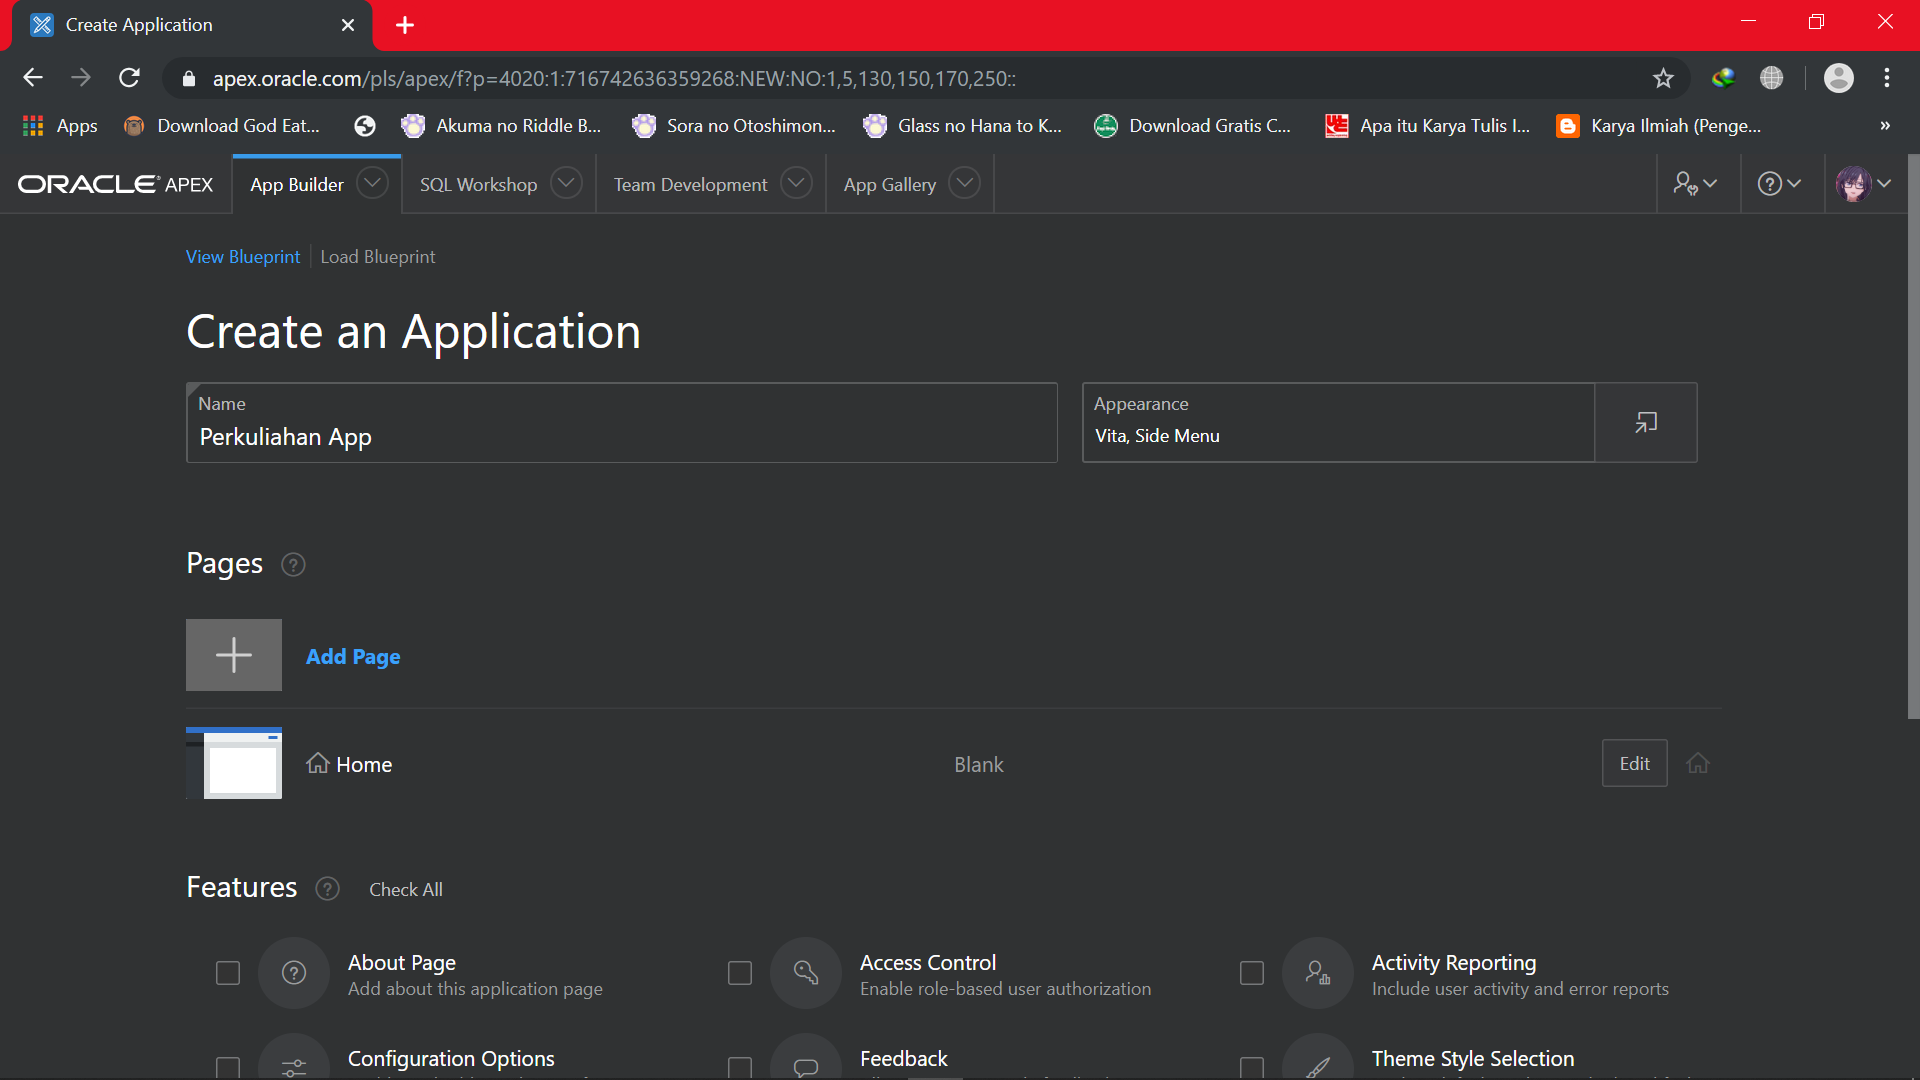
\includegraphics[width=10.5cm]{figures/Screenshot_14.png}
	\caption{Memberi nama Aplikasi}
\end{figure}\\
\\
\\
\item Pada halaman tersebut klik "Add page" pilih "Interactive report".
\begin{figure}[htbp]
	\centering
	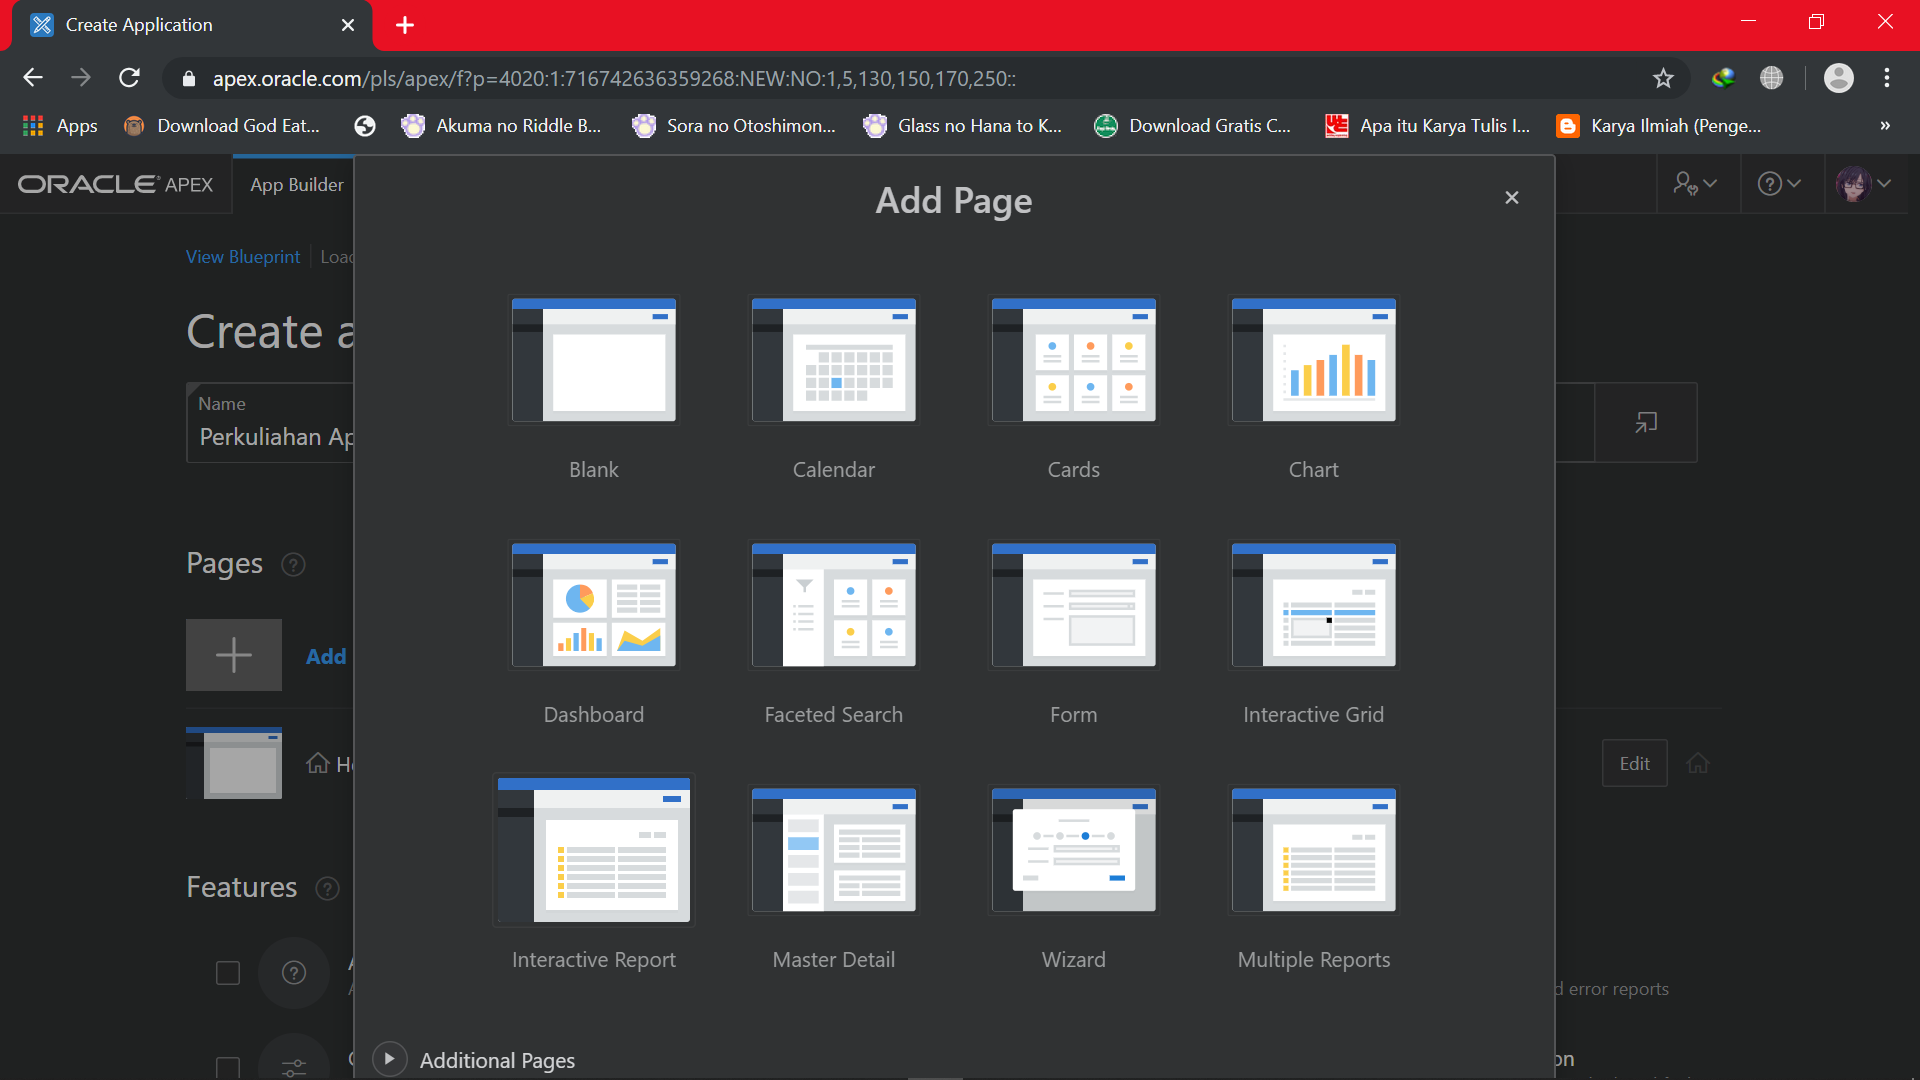
\includegraphics[width=10.5cm]{figures/Screenshot_15.png}
	\caption{Membuat Aplikasi}
\end{figure}
\item Beri nama page "Mahasiswa" lalu pilih tabel mahasiswa. Lakukan hal sama untuk setiap halaman dan tabel.
\begin{figure}[htbp]
	\centering
	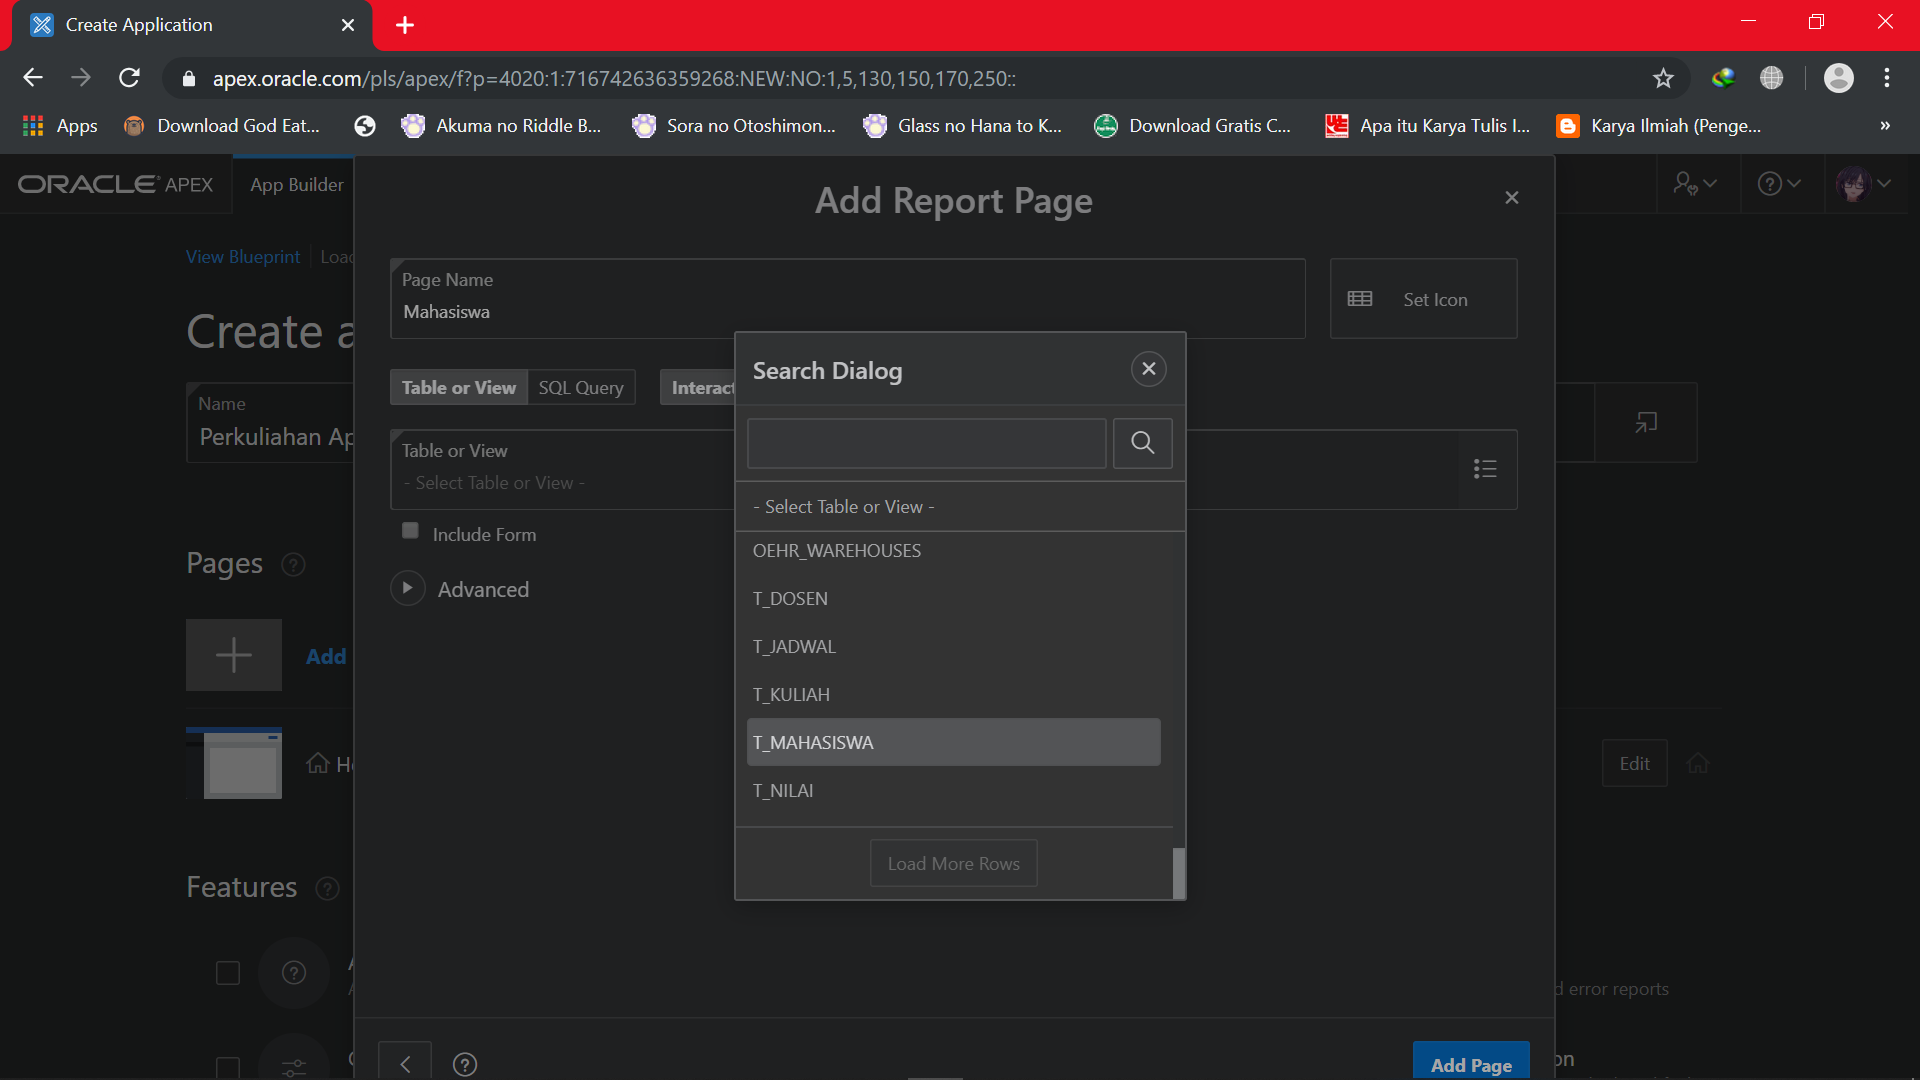
\includegraphics[width=10.5cm]{figures/Screenshot_16.png}
	\caption{Membuat Aplikasi}
\end{figure}
\\
\\
\\
\\
\item Add page sudah selesai.
\begin{figure}[htbp]
	\centering
	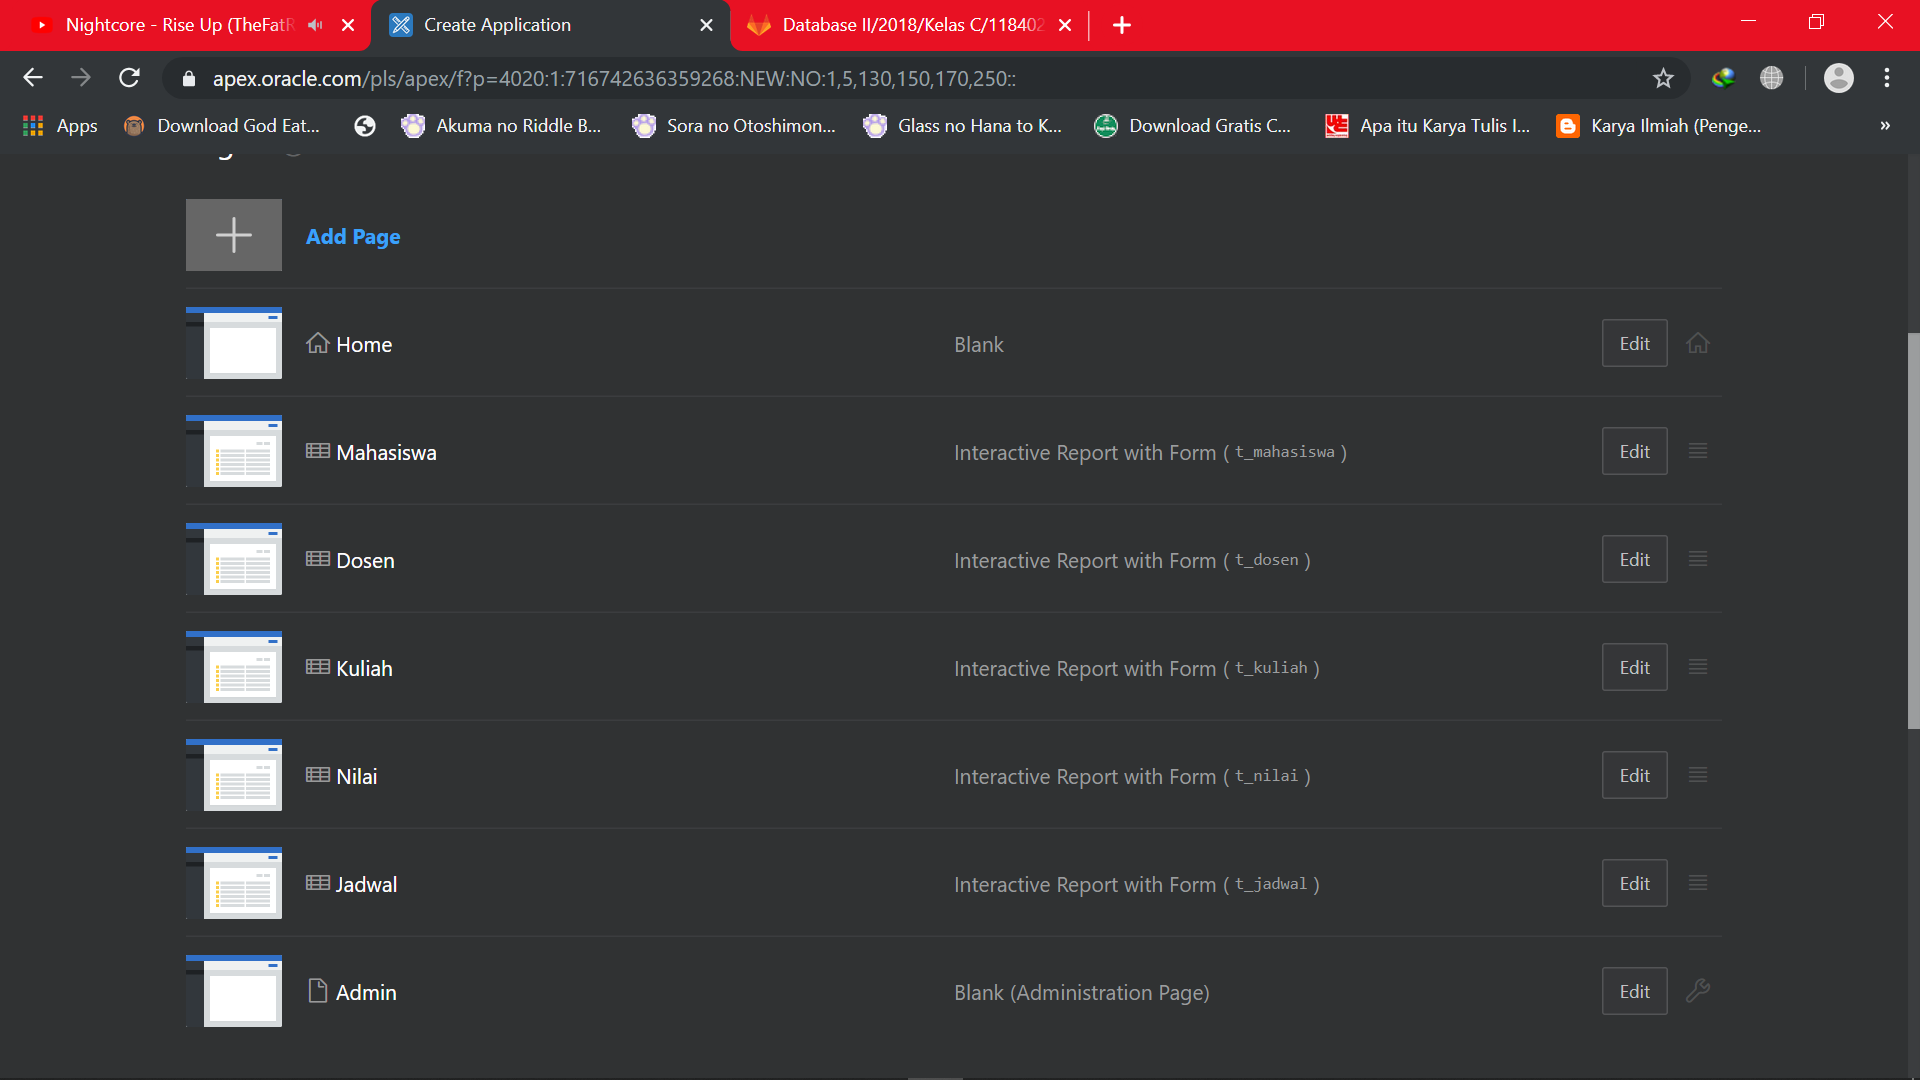
\includegraphics[width=10.5cm]{figures/Screenshot_17.png}
	\caption{Membuat Aplikasi}
\end{figure}
\item Scrool ke bawah dan check all lalu klik "Create Application".
\begin{figure}[htbp]
	\centering
	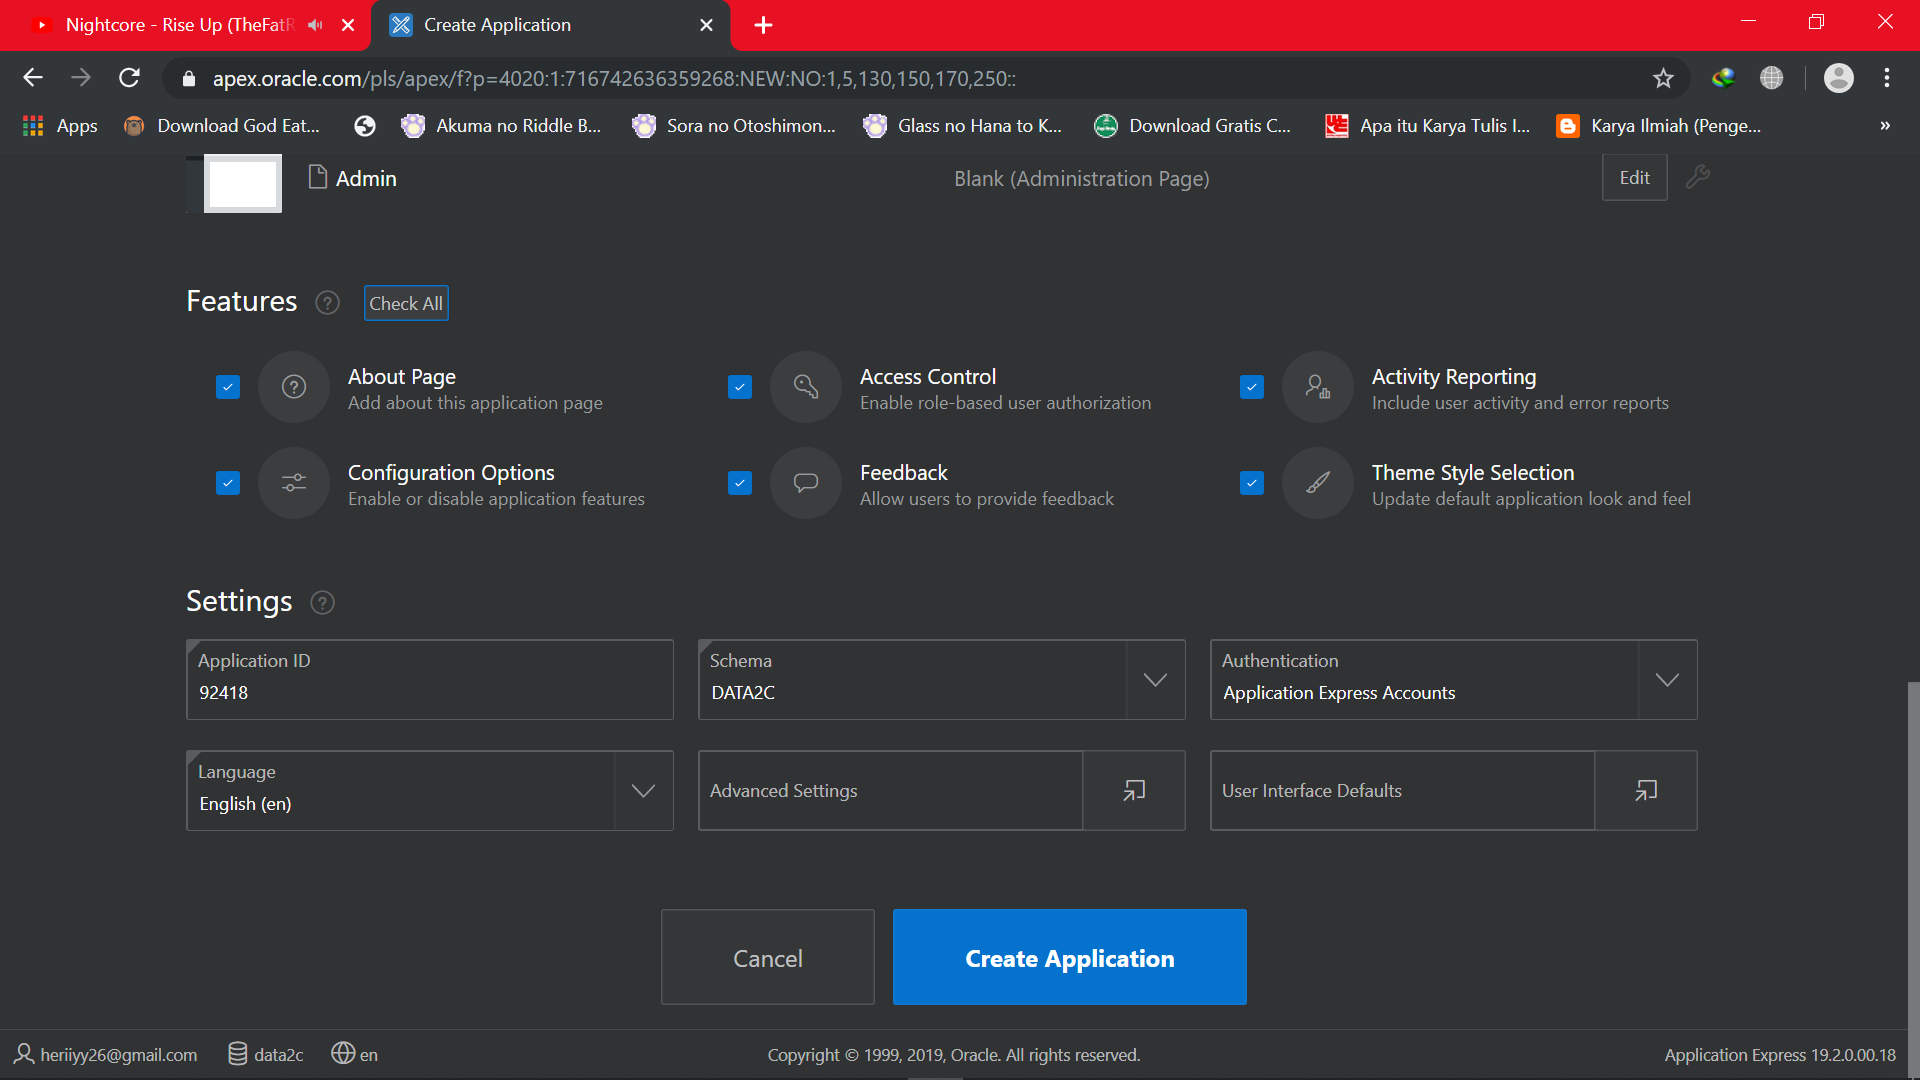
\includegraphics[width=10.5cm]{figures/Screenshot_18.png}
	\caption{Membuat Aplikasi}
\end{figure}\\
\\
\\
\\
\\
\item Buka aplikasi yang telah dibuat tadi dan klik "Run Application".
\begin{figure}[htbp]
	\centering
	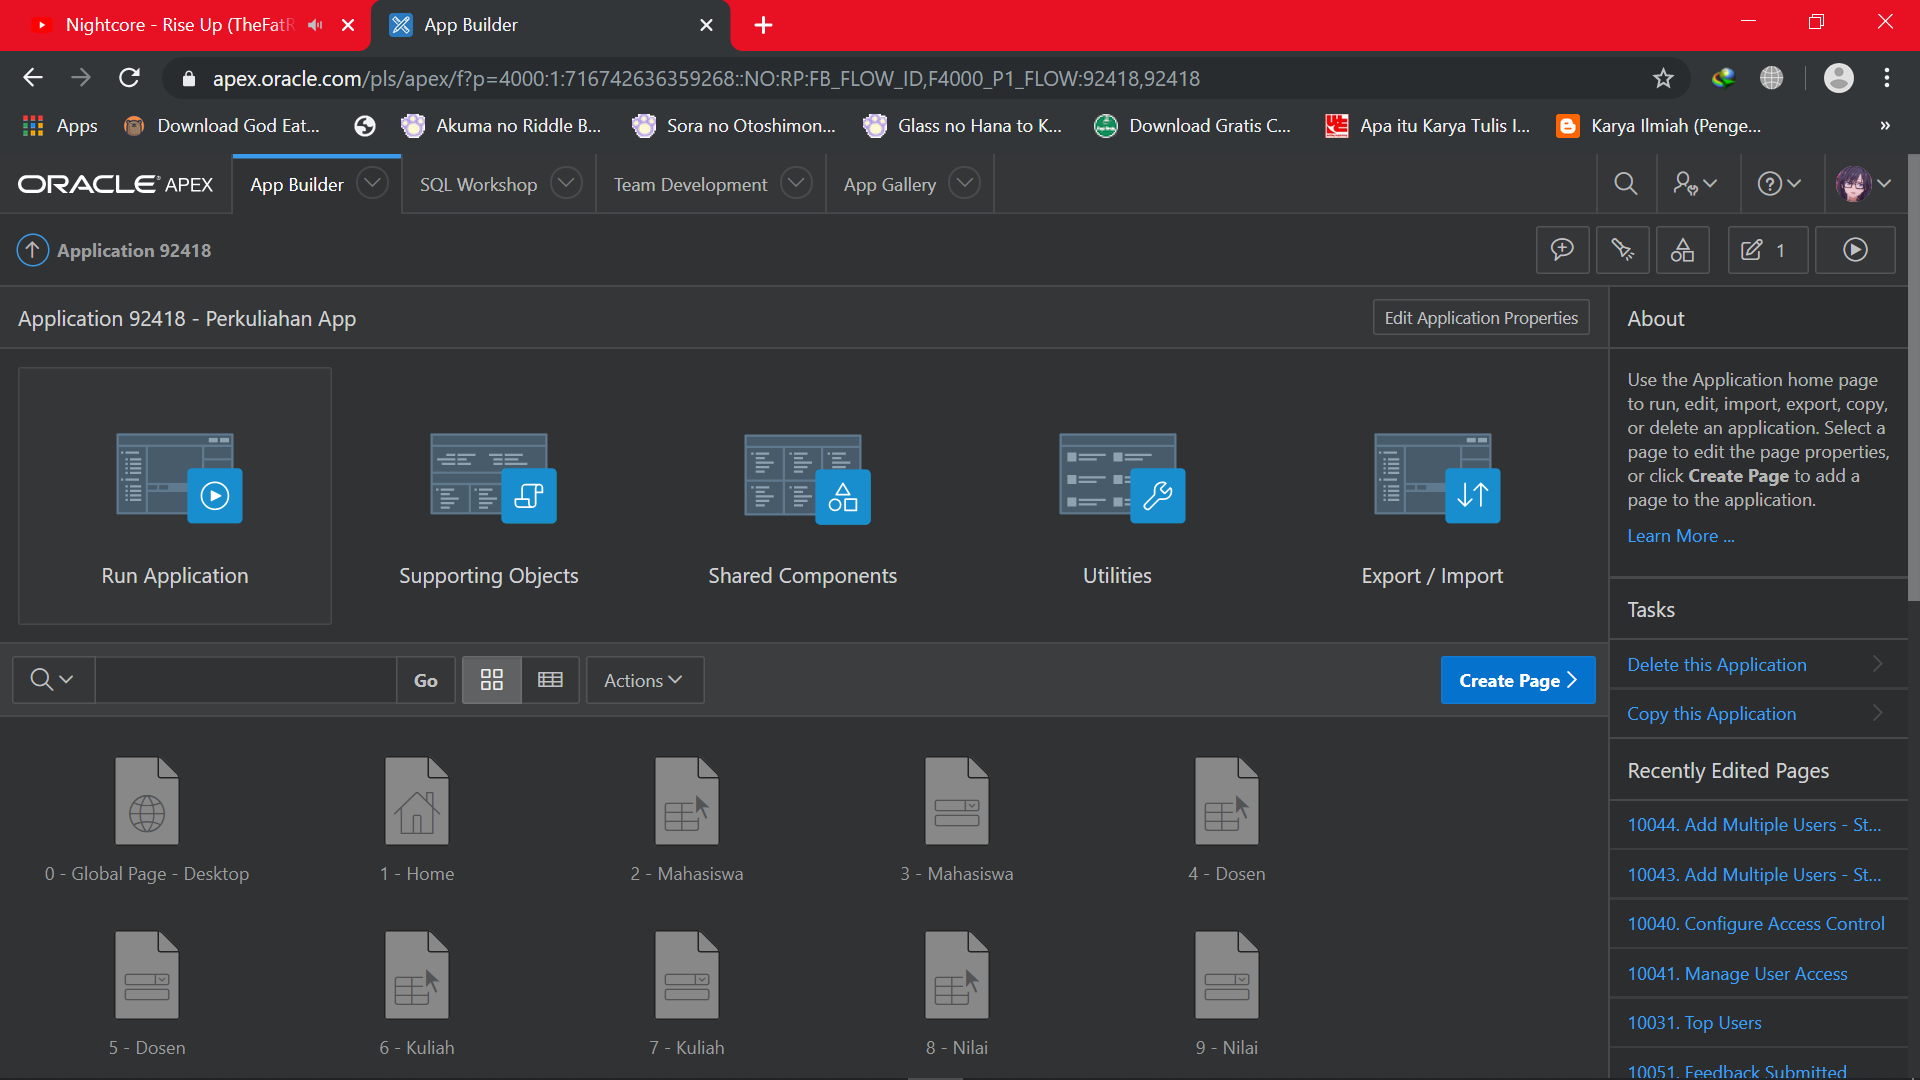
\includegraphics[width=10.5cm]{figures/Screenshot_19.png}
	\caption{Run Application}
\end{figure}
\item Lakukan login ke aplikasi.
\begin{figure}[htbp]
	\centering
	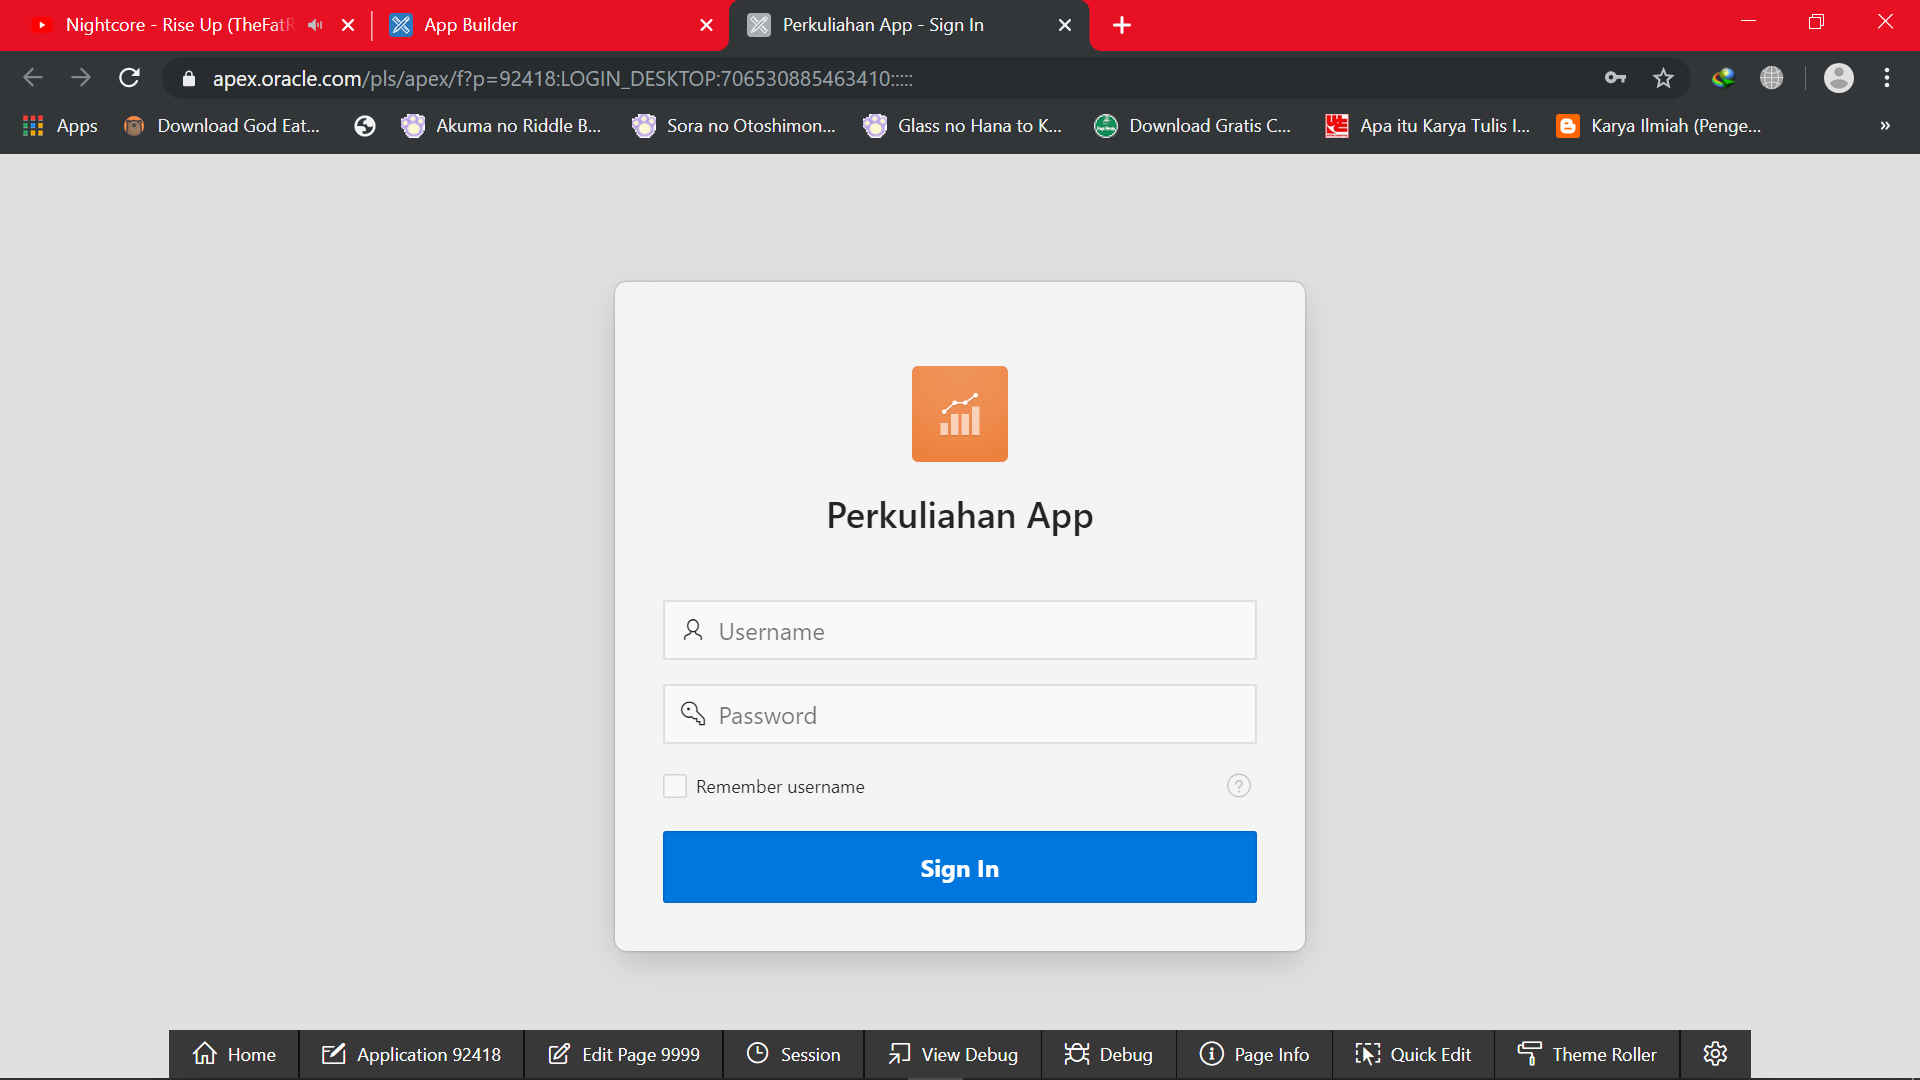
\includegraphics[width=10.5cm]{figures/Screenshot_20.png}
	\caption{Login}
\end{figure}\\
\\
\\
\\
\\
\item Tampilan halaman utama aplikasi.
\begin{figure}[htbp]
	\centering
	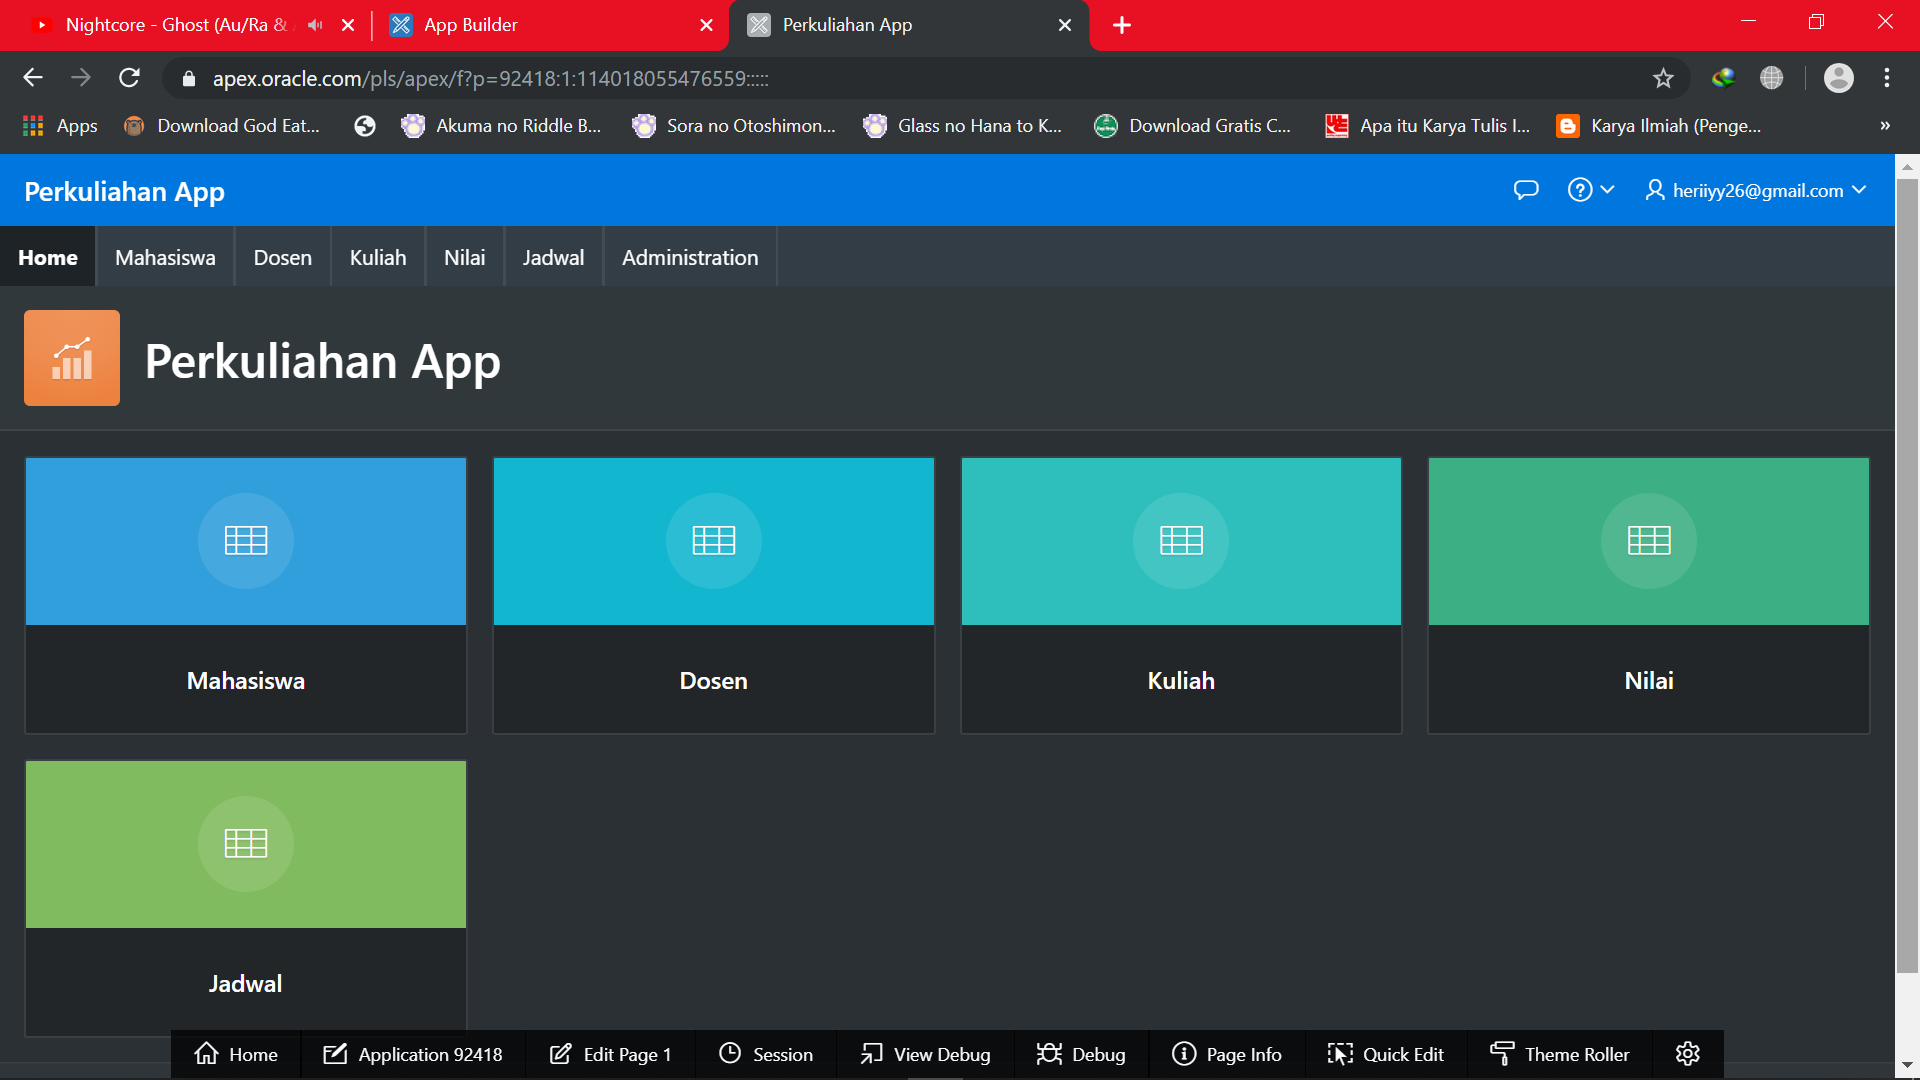
\includegraphics[width=11cm]{figures/Screenshot_21.png}
	\caption{Interface}
\end{figure}
\end{itemize}
\section{Note}
\begin{itemize}
\item Link = https://apex.oracle.com/pls/apex/f?p=92418:1:4720096043710:::::
\item Username = heriiyy26@gmail.com
\item Password = makioshi194
\end{itemize}

\end{document}